\documentclass{article}
\hfuzz=1000pt
\hbadness=10000

\makeatletter
\def\input@path{{style/}}
\makeatother

\usepackage{Main}
\usepackage{scriptStyle}

\usepackage{ThmEnvColored}
%\usepackage{ThmEnvPlain}

\usepackage{AlgEnvColored}
\usepackage{AlgCommands}

\usepackage{MathCommands}

\begin{document}

\begin{titlepage}
    \centering
    \vspace*{3cm}
    \Large\textbf{Numerische Mathematik und Numerische Lineare Algebra in den Datenwissenschaften}

    \vspace{1cm}
    \large
    Prof.\ Dr.\ rer.\ nat.\ Jens\ Starke\\
    Sommersemester 2025

    \vfill
\end{titlepage}

\tableofcontents

\newpage
\vspace*{2cm}
\begin{center}
  \begin{minipage}{0.85\textwidth}
    \small
    Diese Mitschrift basiert auf der gleichnamigen Vorlesung \textit{Numerische Mathematik und 
    Numerische Lineare Algebra in den Datenwissenschaften}, gehalten im Sommersemester 2025 
    an der Universität Rostock.\\[0.5em]
    Alle Rechte an Inhalt und Struktur der Lehrveranstaltung liegen bei dem Modulverantwortlichen, 
    Prof.\ Dr.\ rer.\ nat.\ Jens Starke, sowie der Universität Rostock.\\[0.5em]
    Diese Mitschrift dient ausschließlich zu Lern- und Dokumentationszwecken. Eine kommerzielle Nutzung oder 
    Weiterverbreitung ohne Zustimmung ist nicht gestattet.
  \end{minipage}
\end{center}
\vspace*{5em}
\begin{minipage}{0.85\textwidth}
  \textbf{Literaturempfehlungen:}
  \begin{enumerate}
    \item  Martin Hanku-Bourgeois, Grundlagen der Numerik und des wissenschaftlichen Rechnens, Mathematische Leitfäden,
    Vieweg + Teubner Verlag Wiesbaden, 2009, DOI: \href{https://doi.org/10.1007/978-3-8348-9309-3}{10.1007/978-3-8348-9309-3}
    \item Eberhard Zeidler, Nichtlineare Funktionalanalysis und ihre Anwendung, Springer Spektrum Wiesbaden, 2012, DOI: 
    \href{https://doi.org/10.1007/978-3-658-00289-3_3}{10.1007/978-3-658-00289-3\_3}
  \end{enumerate}
\end{minipage}

% !TeX root = ../script.tex
\section{Wiederholung}
Wir starten mit einer kurzen Wiederholung zur Fixpunktiteration zum Lösen von Gleichungen 
der Form $Tx=x$ durch $x_{n+1}=Tx_n$.

\begin{thmbox}{Satz}[Banach 1922]
    Sei $M$ eine abgeschlossene nichtleere Teilmenge in einem vollständig metrischem Raum $(X,d)$. 
    Sei $T:M\rightarrow M$ eine Selbstabbildung und $k$-kontraktiv, d.h. $d(Tx,Ty)\leq k\cdot d(x,y)\ \forall x,y\in M$ 
    mit $0\leq k < 1$. Dann folgt:
    \begin{enumerate}
        \item Existenz und Eindeutigkeit: die Gleichung $Tx=x$ hat genau eine Lösung, d.h. $T$ hat genau einen 
        Fixpunkt in M.
        \item Konvergenz der Iteration $x_{k+1}=Tx_k$. Die Folge $(x_k)_{k\in\mathbb{N}}$ konvergiert gegen den 
        Fixpunkt $x^*$ für einen beliebigen Startpunkt $x_0\in M$.
        \item Fehlerabschätzung: Für alle $n=0,1,\dotsc$ gilt 
        \begin{itemize}
            \item a-priori: $d(x_n,x^*)\leq k^n(1-k)^{-1}d(x_0,x_1)$
            \item a-posteriori: $d(x_{n+1},x^*)\leq k(1-k)^{-1}d(x_n,x_{n+1})$
        \end{itemize}
        \item Konvergenzrate: Für alle $n\in\mathbb{N}$ gilt $d(x_{n+1},x^*)\leq k\cdot d(x_n,x^*)$
    \end{enumerate}
\end{thmbox}
\textit{Beweis.} 
\begin{enumerate}
    \item[2.] Wir zeigen, dass $(x_n)$ eine Cauchy-Folge ist. Für den Abstand zweier benachbarter Folgeglieder $x_n$ 
    und $x_{n+1}$ gilt
    \[d(x_n,x_{n+1})=d(Tx_{n-1},Tx_n)\leq k\cdot d(x_{n-1},x_n)\leq \dotsc \leq k^n\cdot d(x_0,x_1)\]
    Mehrfache Anwendung der Dreiecksungleichung liefert daher für $n,m\in\mathbb{N}$:
    \begin{align*}
        d(x_n,x_{n+m}) &\leq d(x_n,x_{n+1}) + d(x_{n+1},x_{n+2}) + \dotsc + d(x_{n+m-1}, x_{n+m}) \\
        & \leq (k^n + k^{n+1} + \dotsc + k^{n+m})\cdot d(x_0,x_1) \\
        & \leq k^n(1+k+k^2+\dotsc)\cdot d(x_0,x_1) \\
        & = k^n\cdot(1-k)^{-1}d(x_0,x_1)
    \end{align*}
    Demnach folgt $d(x_n,x_{n+m})\rightarrow 0$ für $n\rightarrow \infty$ und da $X$ vollständig ist 
    konvergiert $(x_n)$ gegen ein $x^*\in X$.
    \item[1.] Da $T$ stetig ist (aufgrund $k$-Kontraktivität) folgt für die konvergente Folge $(x_n)$, dass 
    \[x^* = \lim_{n\rightarrow\infty} x_{n+1} = \lim_{n\rightarrow\infty} Tx_n = Tx^*\]
    Da $M$ abgeschlossen ist existiert also ein Fixpunkt in $M$. \\
    Dieser ist eindeutig, denn für $x,y$ mit $Tx=x$ und $Ty=y$ gilt $d(x,y)=d(Tx,Ty)\leq k d(x,y)$, also $d(x,y)=0$.
    \item[3.] Aus dem Beweis zu 2. haben wir $d(x_n,x_{n+m})\leq k^n(1-k)^{-1}d(x_0,x_1)$, wegen der Stetigkeit 
    der Metrik folgt die a-priori-Fehlerabschätzung aus $m\rightarrow\infty$. \\
    Die a-posteriori-Fehlerabschätzung folgt analog aus dem Ansatz
    \begin{align*}
        d(x_{n+1},x_{n+1+m}) &\leq d(x_{n+1},x_{n+2}) + \dotsc + d(x_{n+m}, x_{n+1+m}) \\
        & \leq (k + \dotsc + k^{m})\cdot d(x_n,x_{n+1}) \\
        & \leq k\cdot(1-k)^{-1}d(x_n,x_{n+1})
    \end{align*}
    \item[4.] Folgt direkt durch $d(x_{n+1},x^*)=d(Tx_n,Tx^*)\leq k\cdot d(x_n,x^*)$ 
\end{enumerate}

\begin{egbox} 
    Wir betrachten das Nullstellenproblem $f:\mathbb{R}\rightarrow\mathbb{R}, x\mapsto \cos x - x = 0$. \\
    Umformung ergibt $\underbrace{\cos x}_{Tx} = x$ und somit die Fixpunktiteration $x_{k+1}=Tx_k=\cos(x_k)$ \\
    \begin{center}
        \begin{tikzpicture}
        \begin{axis}[
            axis lines=middle,
            xmin=0, xmax=2,
            ymin=0, ymax=1.1,
            xtick={1.5708},
            xticklabels={$\frac{\pi}{2}$},
            ytick=\empty,
            grid=none,
            width=9cm,
            height=6cm,
            domain=0:2,
            samples=200,
            clip=false,
            xlabel=$x$,
            ylabel=$y$,
            every axis x label/.style={at={(axis description cs:1.05,0)},anchor=west},
            every axis y label/.style={at={(axis description cs:0,1.05)},anchor=south},
        ]
            
            % Funktionsgraphen
            \addplot[thick, black, domain=0:2] {cos(deg(x))} node[pos=0.6, above right] {$f(x)=\cos x$};
            \addplot[thick, black, domain=0:1.1] {x} node[pos=0.9, above left] {$g(x)=x$};
            
            % Fixpunktlinie
            \addplot[dashed, black] coordinates {(0.739,0) (0.739,0.739)};
            
            % Punkt auf der Diagonalen
            \filldraw[black] (axis cs:0.739,0.739) circle (2pt);
            \node at (axis cs:0.739,-0.06) {$x^*$};
        \end{axis}
        \end{tikzpicture}
    \end{center}
    \underline{Prüfung der Voraussetzungen des Banach'schen FP-Satzes:} \\
    Wir wählen als Einschränkung $M=[0,1]$, dies liefert uns eine Selbstabbildung auf einer abgeschlossenen 
    Teilmenge $M$ des vollständig metrischen Raum $\mathbb{R}$ mit der Abstandsfunktion $ d(x,y) = |x-y|$. \\
    Weiter ist die Abbildung $k$-kontraktiv:  Nach Mittelwertsatz der Differentialrechnung gilt 
    \[|\cos x - \cos y| = \underbrace{|\sin \xi|}_{\leq \sin(1)}\cdot|x-y|\leq \underbrace{0,85}_{=:k}\cdot |x-y|, 
    \quad \text{für } \xi\in[0,1]\]
    Wir können also nach Banach die Existenz und Eindeutigkeit eines Fixpunkt $x^*$ folgern, diesen Fixpunkt 
    finden wir durch die konvergente Folge $x_{k+1}=\cos x_k$. 
\end{egbox}
Wir betrachten im folgenden die Idee der Umwandlung eines Nullstellenproblems in Fixpunkt-Gleichung noch etwas 
allgemeiner. Für eine Gleichung $f(x)=0$ mit $f:\mathbb{R}\rightarrow\mathbb{R}$ haben wir verschiedene Möglichkeiten 
zur Umformung:\\
\begin{enumerate}
    \item[a)] Betrachte $Tx := x-f(x)$ gefolgert aus $f(x)=0\Leftrightarrow -f(x)=0 \Leftrightarrow x-f(x)=x$.
    \item[b)] Betrachte $Tx := x-\omega \cdot f(x)$ mit $\omega\neq 0$ (lineare Relaxation)
    \item[c)] Betrachte $Tx:=x-\omega \cdot g(f(x))$ mit $\omega \neq 0$ und geeigneter Funktion $g$ 
    (nichtlineare Relaxation). Wenn $g(0)\neq 0$ dann betrachte $Tx:=x-\omega\cdot(g(f(x))+g(0))$
    \newpage
    \item[d)] Betrachte $Tx:=x-(f'(x))^{-1} f(x)$ (Newtonverfahren) \\
    Newton hat teils Probleme, bei falschen Startwerten: \\
    \begin{center}
        \begin{tikzpicture}

        % Startwert
        \pgfmathsetmacro{\xzero}{1.5}
        \pgfmathsetmacro{\fxzero}{\xzero * exp(-\xzero^2)}
        \pgfmathsetmacro{\dfxzero}{exp(-\xzero^2) * (1 - 2 * \xzero^2)}
        \pgfmathsetmacro{\xone}{\xzero - \fxzero / \dfxzero}

        \pgfmathsetmacro{\fxone}{\xone * exp(-\xone^2)}
        \pgfmathsetmacro{\dfxone}{exp(-\xone^2) * (1 - 2 * \xone^2)}
        \pgfmathsetmacro{\xtwo}{\xone - \fxone / \dfxone}

        \pgfmathsetmacro{\fxtwo}{\xtwo * exp(-\xtwo^2)}
        \pgfmathsetmacro{\dfxtwo}{exp(-\xtwo^2) * (1 - 2 * \xtwo^2)}
        \pgfmathsetmacro{\xthree}{\xtwo - \fxtwo / \dfxtwo}

        \begin{axis}[
            axis lines=middle,
            xmin=-.1, xmax=3,
            ymin=-0.4, ymax=0.4,
            samples=300,
            width=12cm,
            height=7cm,
            domain=-.1:3,
            clip=false,
            xtick=\empty,
            ytick=\empty,
        ]
        
            % Funktion f(x) = x*exp(-x^2)
            \addplot[thick, black] {x * exp(-x^2)} node[pos=0.2, above left] {$f(x)$};

            % Punkte (x0, x1, x2)
            \addplot[only marks, mark=*, mark size=2pt] coordinates {
            (\xzero, \fxzero)
            (\xone, \fxone)
            (\xtwo, \fxtwo)
            };
            
            % Beschriftung der x-Werte
            \node at (axis cs:\xzero,-0.08) {$x_0$};
            \node at (axis cs:\xone,-0.08) {$x_1$};
            \node at (axis cs:\xtwo,-0.08) {$x_2$};

            % Tangente bei x0
            \addplot[dashed, domain=\xzero-1:\xzero+1] {\fxzero + \dfxzero*(x - \xzero)};
            % Tangente bei x1
            \addplot[dashed, domain=\xone-1:\xone+1] {\fxone + \dfxone*(x - \xone)};
            % Tangente bei x2
            \addplot[dashed, domain=\xtwo-1:\xtwo+1] {\fxtwo + \dfxtwo*(x - \xtwo)};
            
            % Pfeile
            %\draw[->, thick] (axis cs:\xzero,\fxzero) -- (axis cs:\xone,0);
            %\draw[->, thick] (axis cs:\xone,\fxone) -- (axis cs:\xtwo,0);
            %\draw[->, thick] (axis cs:\xtwo,\fxtwo) -- (axis cs:\xthree,0);
            
            \node at (axis cs:\xthree,-0.08) {$x_3$};

        \end{axis}
        \end{tikzpicture}
    \end{center}
    \item[e)] Betrachte $Tx:=h^{-1}(f(x)-g(x))$, wobei $f(x)=h(x)+g(x)$ (Splitting-Verfahren) 
\end{enumerate}
\section{Iteratives Vorgehen zur Lösung linearer Gleichungssysteme}
\subsection{Splittingverfahren}
Gegeben sei das LGS $Ax=b$ für $A\in\mathbb{K}^{n\times n}, b\in\mathbb{K}^n, x\in\mathbb{K}^n$, 
wobei $\mathbb{K}\in\{\mathbb{R}, \mathbb{C}\}$. Wir wollen dieses LGS nun in ein FP-Problem umformen, 
sei hierfür $A$ nicht singulär (sonst nicht lösbar). \\
Wir schreiben $A=M-N$, wobei $M$ invertierbar und häufig sogar eine Diagonalmatrix ist 
(damit $M$ leicht zu invertieren ist). Dies liefert:
\[Ax = b \Leftrightarrow (M-N)x=b \Leftrightarrow Mx=Nx+b x=\underbrace{M^{-1}\cdot(Nx+b)}_{\Tilde{T}x}\]
$\Tilde{T}$ ist affin-linear. Wir erhalten also unser FP-Problem $x=\Tilde{T}x=Tx+c$ 
mit $T=M^{-1}N$ und $c=M^{-1}b$ \\ \\

\algobox{Splittingverfahren}{
\begin{algorithm}[H]
    \SetAlgoNoLine
    \InitTe{$A=M-N$ mit $N\in GL(n,\mathbb{K})$}{}
    \SetAlgoLined
    Wähle $x^{(0)}\in\mathbb{K}^n$ beliebig \\
    \ForTe{$k=0,1,\dotsc$}{
        löse $Mx^k=Nx^{k-1}+b$} 
    \SetAlgoNoLine
    \UntilTe{stop (beliebiges Stopkriterium)}{}
\end{algorithm}
}
Konvergenz dieses Algorithmus folgt aus Banachschen Fixpunktsatz.

\begin{rembox}
    Nach gleicher Überlegung lässt sich auch unser obiges Splittingverfahren für Nullstellenbestimmung herleiten:
    \[f(x)=0\Leftrightarrow h(x)+g(x):=f(x) = 0 \Leftrightarrow h(x)=f(x)-g(x) \Leftrightarrow x=h^{-1}(f(x)-g(x))\]
\end{rembox}
\textit{Wiederholung:} Eine Matrixnorm ist eine Norm auf dem Vektorraum der Matrizen, 
d.h. $\|\cdot\|:\mathbb{K}^{n\times n}\rightarrow \mathbb{R}$, bereits bekannte Matrixnormen sind:
\begin{itemize}
    \item Frobeniusnorm: $\|A\|_F := \left(\displaystyle \sum_{i,j}|a_{ij}|^2\right)^{1/2}$
    \item Spaltensummennorm $\|A\|_1:=\max_j \sum_i |a_{ij}|$
    \item Zeilensumennorm $\|A\|_\infty:=\max_i \sum_j |a_{ij}|$
    \item Spektralnorm $\|A\|_2:=\sqrt{\lambda_{max}(A^HA)}$, \qquad $(A^H := \overline{A}^T)$
\end{itemize}
Im allgemeinen induziert eine Vektornorm auch immer eine Matrixnorm, diese nennen wir auch Operatornorm:
\[\|A\|:=\max_{\|x\|=1}\|Ax\|\]
Die oben aufgelisteten Normen $\|\cdot\|_1,\|\cdot\|_2$ und $\|\cdot\|_\infty$ sind die Operatornormen zu 
der jeweiligen $p$-Normen. \\ \\
Eine Norm $\|\cdot\|$ auf $\mathbb{K}^{n\times n}$ heißt submultiplikativ, falls $\|AB\|\leq\|A\|\cdot\|B\|$ 
und sie heißt verträglich mit einer Vektornorm $\|\cdot\|_V$, falls $\|Ax\|_V\leq \|A\|\cdot\|x\|_V$. \\
Operatornormen sind immer submultiplikativ und verträglich zu der Vektorrnorm, aus welcher sie abgeleitet wurden.
\begin{thmbox}{Satz}
    Ist $\vertiii{\cdot}$ eine Norm auf $\mathbb{K}^{n\times n}$, die mit einer Vektornorm verträglich ist, 
    und ist $\vertiii{M^{-1}N}<1$, dann konvergiert der Algorithmus für jedes für jedes $x^{(0)}\in\mathbb{K}^n$ 
    gegen $A^{-1}b$, d.h. gegen die Lösung des linearen Gleichungssystems $Ax=b$.
\end{thmbox}
\textit{Beweis.} Sei $\tilde{T}(x) := Tx + c$ mit $T=M^{-1}N$ und $c=M^{-1}b$.\\
Offensichtlich gilt $\tilde{T}:\mathbb{K}^n\rightarrow\mathbb{K}^n$, sowie 
\[\|\tilde{T}(x)-\tilde{T}(y)\| = \|Tx-Ty\|\leq \|T\|\cdot\|x-y\|\]
Da $\|T\|=\|M^{-1}N\|<1$ ist $\tilde{T}$ eine $k$-kontraktive Selbstabbildung und somit konvergiert 
die Folge $(x^k)$ aus dem Algorithmus gegen den eindeutigen Fixpunkt $x^*$ mit $\tilde{T}(x^*)=x^*$. \\ 
Einsetzen der Definition von $\tilde{T}$ liefert:
\[x^*=Tx+c=M^{-1}(Nx+b)\Rightarrow Mx=Nx+b \Rightarrow Ax=(M-N)x=b\]
\begin{thmbox}{Korollar}
    Sei $A$ invertierbar, so konvergiert der obige Algorithmus genau dann für alle Startwerte $x^{(0)}\in\mathbb{K}^n$ 
    gegen $x^*=A^{-1}b$, wenn für den Spektralradius $\rho(T)=\max\{|\lambda|:\lambda\in\sigma(T)\}$ 
    die Ungleichung $\rho(T)<1$ erfüllt ist.
\end{thmbox}
\textit{Beweis.} \\
$\Leftarrow:$ Falls $\rho(T)<1$ dann existiert eine Norm $\|\cdot\|_\varepsilon$ auf $\mathbb{K}^n$ 
und eine dadurch induzierte Operatornorm $\vertiii{\cdot}_\varepsilon$ auf $\mathbb{K}^{n\times n}$ 
mit $\vertiii{T}_\varepsilon \leq \rho(T) + \varepsilon < 1$ für $\varepsilon$ klein genug. \\
Satz 2.2 liefert dann die Konvergenz des Algorithmus. \\ \\
$\Rightarrow:$ Angenommen $\rho(T)\geq 1$, d.h. es existiert ein Eigenwert $\lambda$ von $T$ 
mit $|\lambda|\geq 1$ und zugehörigem Eigenvektor $z$. Für $x^{(0)}=x^*+z$ und festes $k$ sich der Iterationsfehler
\[x^{(k)}-x^* = Tx^{(k-1)}+c-x^* = Tx^{(k-1)}-Tx^* = T(x^{(k-1)}-x^*)\]
Induktiv folgt dann $x^{(k)}-x^* = T^k(x^{0}-x^*)=T^kz=\lambda^kz$, demnach gilt 
$\|x^{(k)}-x^*\|=|\lambda^k|\cdot\|z\|$.
Für größer werdendes $k$ kann $x^{(k)}$ also nicht gegen $x^*$ konvergieren. \\ \\
\begin{thmbox}{Satz}
    Unter gleichen Voraussetzungen des obigen Korollars gilt 
    \[\max_{x^{(0)}\in\mathbb{K}^n} \limsup_{k\rightarrow \infty} \|x^*-x^{(k)}\|^{1/k}=\rho(T)\]
\end{thmbox}
\textit{Beweis.}
Aus dem Beweis von Korollar 2.3 sehen wir
\[\max_{x^{(0)}\in\mathbb{K}^n} \limsup_{k\rightarrow \infty} \|x^*-x^{(k)}\|^{1/k}
\geq\limsup_{k\rightarrow\infty} \|T^kz\|^{1/k}=\limsup_{k\rightarrow\infty}|\lambda|\cdot\|z\|^{1/k}
=|\lambda|=\rho(T)\]
Für jeden Startwert $x^{(0)}\in\mathbb{K}^n$ gilt nun 
\[\|x^{(k)}-x^*\|_\varepsilon = \|T^k(x^{(0)}-x^*)\|_\varepsilon
\leq \|T\|_\varepsilon^k\cdot \|x^{(0)}-x^*\|_\varepsilon\]
Da im $\mathbb{K}^n$ alle Normen äquivalent sind, also inbesondere auch $\|\cdot\|_\varepsilon$ 
und $\|\cdot\|$, exisitert eine Konstante $c_\varepsilon>0$, so dass
\[\|x^{(k)}-x^*\|^{1/k}\leq\left(c_\varepsilon\cdot\|x^{(k)}-x^*\|_\varepsilon\right)^{1/k}
\leq \|T\|_\varepsilon\cdot\left(c_\varepsilon\cdot\|x^{(0)}-x^*\|_\varepsilon\right)^{1/k}
\xrightarrow{k\rightarrow\infty} \|T\|_\varepsilon\]
Folglich ist 
\[\varrho(T) \le \max_{x^{(0)}} \limsup_{k\rightarrow \infty} \|x^{(k)}-x^*\|^{1/k}\le \vertiii{T}_\varepsilon\]
\qed
Dieser Satz ermöglicht es nun einen sinnvollen Begriff der Konvergenzrate zu definieren:
\begin{defbox} \\
    Die Zahl $\varrho(T)$ heißt (asymptotischer) Konvergenzfaktor von der Iteration $x^{(k)}=Tx^{(k-1)}+c$. \\
    Die (asymptotische) Konvergenzrate lässt sich dadurch ausdrücken mit $r=-\log_{10}\varrho(T)$
\end{defbox}
Mittels der Zerlegung $A=D+L+R$, wobei $D$ die Dianale, $L$ die untere (linke) Hälfte 
und $R$ die obere (rechte) Hälfte der Matrix $A$ sind, erhalten wir einen Spezialfall der Splitting-Vefahren. \\
Durch die Wahl $M=D$ und $N=L+R$ ergibt sich $x^{(k+1)}=D^{-1}(b - (L+R)x^{(k)})$, bzw. in algorithmischer Form:\\ \\
\algobox{Jacobi / Gesamtschritt Verfahren}{
    Gegeben sei das Lineare Gleichungssystem $Ax=b$ mit $a_{ii}\neq 0$. \\
    \begin{algorithm}[H]
        \SetAlgoNoLine
        \InitTe{Wähle beliebigen Startvektor $x^{(0)}\in\mathbb{K}^n$}{}
        \SetAlgoLined
        \ForTe{$k=1,0,\dotsc$}{
            \ForTe{$i=1,\dotsc,n$}{
                $x_i^{(k+1)}\leftarrow \dfrac{1}{a_{ii}}\left(b_i - \displaystyle\sum_{i\neq j}a_{ij}x_j^{(k)}\right)$
            } \EndTe{}{}
        } 
        \SetAlgoNoLine
        \UntilTe{stop (beliebiges Stopkriterium)}{}
    \end{algorithm}
}
Die zugehörige Iterationsmatrix ist hierbei $J=M^{-1}N = D^{-1}(L+R)$ 
und nennt sich (beim Jacobi Verfahren) Gesamtschrittoperator. \\ \\
Einen weitere Version des Splitting-Verfahren ergibt sich durch die Wahl $M=D-L$ und $N=R$.
Hierbei bildet $D-L$ eine obere Dreiecksmatrix und die Inversion ergibt sich mittels Vorwärtssubstitution: \\ \\
\algobox{Gauss-Seidel / Einzelschritt Verfahren}{
    Gegeben sei das Lineare Gleichungssystem $Ax=b$ mit $a_{ii}\neq 0$. \\
    \begin{algorithm}[H]
        \SetAlgoNoLine
        \InitTe{Wähle beliebigen Startvektor $x^{(0)}\in\mathbb{K}^n$}{}
        \SetAlgoLined
        \ForTe{$k=1,0,\dotsc$}{
            \ForTe{$i=1,\dotsc,n$}{
                $x_i^{(k+1)}\leftarrow \dfrac{1}{a_{ii}}\left(b_i - \displaystyle\sum_{j<i}a_{ij}x_j^{(k+1)}
                -\sum_{j>i}a_{ij}x_j^{(k)}\right)$
            } \EndTe{}{}
        } 
        \SetAlgoNoLine
        \UntilTe{stop (beliebiges Stopkriterium)}{}
    \end{algorithm}
}
Die hier erhaltene Iterationsmatrix nennen wir Einzelschrittoperator $L=(D-L)^{-1}R$
Mittels der Zeilensumennorm erhalten wir nun ein leicht prüfbares Konvergenzkriterium:
\begin{thmbox}{Satz}
    Ist $A\in\text{GL}_n(\mathbb{K})$ strikt diagonaldominant, d.h. $|a_{ii}| > \sum_{j\neq i} |a_{ij}|$, 
    dann konvergieren Jordan und Gauss-Seidel Verfahren für alle Startwerte $x^{(0)}\in\mathbb{K}^n$ gegen 
    die eindeutige Lösung von $Ax=b$.
\end{thmbox}
\textit{Beweis.} \\
Da $A$ strikt diagonaldominant ist, muss $a_ii \neq 0$ und damit sind beide Verfahren wohldefiniert.
\begin{enumerate}
    \item[a)] Jacobi Verfahren: Für die Iterationsmatrix gilt
    \[\|J\|_\infty = \|D^{-1}(L+R)\|_\infty = \max_{i\in[n]}\dfrac{1}{|a_{ii}|}\sum_{j\neq i}|a_{ij}| =: q < 1\]
    Nach Satz 2.2 folgt damit die Konvergenz des Jacobi Verfahren.
    \item[b)] Gauss-Seidel Verfahren: Um $\|L\|_\infty < 1$ zu zeigen, nutzen wir, 
    dass die Zeilensumennorm die Operatornorm induziert durch die Maximumsnorm ist, d.h.
    \[\|L\|_\infty = \max_{\|x\|_\infty = 1} \|Lx\|_\infty\]
    Sei nun $y=Lx$ für ein $x\in\mathbb{K}^n$ mit $\|x\|_\infty=1$. \\
    Induktiv folgt nun $y_i \le q < 1$, der Induktionsanfang folgt dabei aus dem Beweisteil a). \\
    Unter der Induktionsvoraussetzung gilt für $j<i$, dass $|y_j|\le q$ und damit:
    \begin{align*}
        \|y_i\| &\le \dfrac{1}{|a_{ii}|}\left(\sum_{j<i}|a_{ij}|\cdot\underbrace{|y_j|}_{\le q}
        +\sum_{j>i}|a_{ij}|\cdot\underbrace{|x_j|}_{\le \|x\|_\infty}\right) \\
        &\le \dfrac{1}{|a_{ii}|}\left(\sum_{j<i}|a_{ij}|\cdot q+\sum_{j>i}|a_{ij}|\cdot \|x\|_\infty\right) \\
        & < \dfrac{1}{|a_{ii}|}\left(\sum_{j<i}|a_{ij}|+\sum_{j>i}|a_{ij}|\right) \\
        & = \dfrac{1}{|a_{ii}|}\sum_{j\neq i} |a_{ij}| \\
        & = q
    \end{align*}
    Da dies für alle Einträge von $y$ gilt folgt $\|y\|_\infty = \|Lx\|_\infty \leq q$ für alle $x$ 
    mit $\|x\|_\infty=1$ und damit $\|L\|_\infty \leq q < 1$ 
    \qed
\end{enumerate}
\begin{egbox}
    Gegeben sei das LGS $Ax=b$ mit 
    \[A = \begin{pmatrix}
        2 & 0 & 1 \\ 1 & -4 & 1 \\ 0 & -1 & 2
    \end{pmatrix}, 
    \quad b=\begin{pmatrix}
        1 \\ 4 \\ -1
    \end{pmatrix}\]
    Dieses System hat die eindeutige Lösung $x^* = (1, -1, -1)^T$. \\
    Durch die Wahl $x^{(0)}=(1,1,1)^T$ erhalten wir beim Jacobi Verfahren:
    \begin{align*}
        x^{(1)} &= D^{-1}(b-(L+R)x^{(0)}) = \begin{pmatrix}
            \tfrac{1}{2} & 0 & 0 \\ 0 & -\tfrac{1}{4} & 0 \\ 0 & 0 & \tfrac{1}{2}
        \end{pmatrix} \cdot \left[\begin{pmatrix}
            1 \\ 4 \\ -1
        \end{pmatrix}-\begin{pmatrix}
            0 & 0 & 1 \\ 1 & 0 & 1 \\ 0 & -1 & 0
        \end{pmatrix}\cdot\begin{pmatrix}
            1 \\ 1 \\ 1
        \end{pmatrix}\right] = \begin{pmatrix}
            0 \\ -\tfrac{1}{2} \\ 0
        \end{pmatrix} \\
        x^{(2)} &= D^{-1}(b-(L+R)x^{(1)}) = \begin{pmatrix}
            \tfrac{1}{2} & 0 & 0 \\ 0 & -\tfrac{1}{4} & 0 \\ 0 & 0 & \tfrac{1}{2}
        \end{pmatrix} \cdot \left[\begin{pmatrix}
            1 \\ 4 \\ -1
        \end{pmatrix}-\begin{pmatrix}
            0 & 0 & 1 \\ 1 & 0 & 1 \\ 0 & -1 & 0
        \end{pmatrix}\cdot\begin{pmatrix}
            0 \\ -\tfrac{1}{2} \\ 0
        \end{pmatrix}\right] = \begin{pmatrix}
            \tfrac{1}{2} \\ -1 \\ -\tfrac{3}{4}
        \end{pmatrix} \\
        \vdots\quad&
    \end{align*}
\end{egbox}
\subsection{Gradientenverfahren}
\subsubsection{Gradientenverfahren für Optimierung} Eine Funtion $f:\mathbb{K}^n\rightarrow \mathbb{K}$ soll minimiert werden. 
Von einem Startpunkt $x^{(0)}$ ausgehen bewegen wir uns nun Stück für Stück in Richtung des steilsten Abstiegs, 
intuitiv sollten wir so ein Minimum finden. \\
Als Iterationsvorschrift ergibt sich $x^{(k+1)} = x^{(k)}+\alpha^{(k)}\cdot d^{(k)}, \quad k=0,1,\dotsc$\\
dabei ist $\alpha^{(k)}>0$ die Schrittweite und Abstriegsrichtung $d^{(k)}\in\mathbb{K}^n$.
(Eine typische Wahl der Abstriegsrichtung ist $d^{(k)}=-\partial f/\partial x (x^{(k)})=-\nabla f(x^{(k)})$) \\
Das Ziel ist des Verfahren ist es, dass sich der Wert von $f$ in jedem Schritt verbessert, 
d.h. $f(x^{(k+1)})<f(x^{(k)})$. 
Es ergibt sich ein 1-dim. Optimierungsproblem für die Schrittweite $\alpha^{(k)}$:
\[\alpha^{(k+1)}=\min_{\alpha\neq 0}\{f(x^{(k)}+\alpha\cdot d^{(k)})\}\]
Ein Nachteil des Verfahrens ist die mögliche Entstehung oszillierender Pfade (\glqq Zick-Zack-Verhalten\grqq{}) 
aufgrund unvorteilhafter Richtungen.\\ \\
\subsubsection{Das Verfahren der konjugierten Gradienten}
Die obige Idee kann zur effizienten Lösung linearer Gleichungssysteme genutzt werden.
Gegeben sei das LGS $Ax=b$ mit $A\in\mathbb{K}^{n\times n}$ hermitisch, 
d.h. $a_{ij}=\overline{a_{ji}}$ (hieraus folgt inbesondere, dass die Hauptdiagonale reell ist). 
Zur Lösung wird hierbei die Minimierung des quaratischen Funktionals 
\[\phi(x)=\tfrac{1}{2}x^* Ax - x^*b\]
Sollte eine Lösung $\hat{x}=A^{-1}b$ des LGS $Ax=b$ exisitieren, so gilt für alle $x\in\mathbb{K}^{n\times n}$:
\begin{align*}
    \phi(x)-\phi(\hat{x}) &= \tfrac{1}{2}x^* Ax - x^*b - (\tfrac{1}{2}\hat{x}^* A\hat{x} - \hat{x}^*b) \\
    &\ \ \vdots \\
    &= \tfrac{1}{2} (x-\hat{x})^*A(x-\hat{x}) \geq 0
\end{align*}
Die Funktion hat demnach ein eindeutiges Minimum bei $\hat{x}$.
\begin{defbox}
    Ist $A\in\mathbb{K}^{n\times n}$ hermitisch und pos. definitiv, dann wird durch $\|x\|_A=\sqrt{x^*Ax}, 
    x\in\mathbb{K}^{n\times n}$ eine Norm in $\mathbb{K}^n$ definiert, die sogenannte Energienorm. 
    Zur Energienorm gehört ein inneres Produkt, nämlich $\langle x,y\rangle_A=x^*Ay, x,y\in\mathbb{K}^n$.
    Mithilfe dieser Definition und obiger Erkentniss ergibt sich die Abweichung des Funktionals von seinem Minimum:
    \[\phi(x)-\phi(\hat{x}) = \tfrac{1}{2}\|x-\hat{x}\|^2_A\]
\end{defbox}
\textbf{geometrische Interpretation:} Der Graph von $\phi$ bezüglich der Energienorm ist ein kreisförmiger Parabloid, 
welcher über dem Mittelpunkt $\hat{x}$ liegt. \\
\textbf{Idee:} Konstruktion eines Verfahrens, welches die Lösung $\hat{x}$ von $Ax=b$ iterativ approximiert, 
indem das Funktional $\phi$ zukzessiv minimiert wird: \\
Zur aktuellen Iteration $x^{(k)}$ wird die Suchrichtung $d^{(k)}\neq 0$ bestimmt, und die neue Iterierte 
$x^{(k+1)}$ über den Ansatz 
\[x^{(k+1)} = x^{(k)} + \alpha\cdot d^{(k)} \tag{3}\]
bestimmt. Es gilt
\[\phi(x^{(k)}+\alpha d^{(k)}) = \phi(x^{(k)}) + \alpha d^{(k)}A x^{(k)} + 
\tfrac{1}{2}\alpha^2 {d^{(k)}}^*Ad^{(k)}-2{d^{(k)}}^*\cdot b \tag{4}\]
Durch Differentiation und Null setzen der Ableitung ergibt sich die Schrittweite $\alpha^{(k)}$:
\[\alpha^{(k)}=\dfrac{{r^{(k)}}^* d^{(k)}}{{d^{(k)}}^* A d^{(k)}},\qquad \text{mit } r^{(k)}=b-Ax^{(k)} \tag{5}\]
Weiter ergibt sich die Suchrichtung $d^{(k+1)}$:
\begin{align*}
    d^{(k+1)}&=r^{(k+1)} + \beta^{(k)}d^{(k)},\quad \langle d^{(k+1)}, d^{(k)}\rangle_A = 0\tag{6}\\
    \text{mit } \beta^{(k)} &= -\dfrac{r^{(k+1)}Ad^{(k)}}{d^{(k)}Ad^{(k)}} \tag{7}
\end{align*}
Die Gleichungen (5) und (7) sind wohldefiniert, wenn ${d^{(k)}}^*Ad^{(k)}\neq 0$, aufgrund der positiv Definitheit 
von $A$ ist dies genau dann der Fall wenn $d^{(k)}\neq 0$. 
Nach (6) ist $d^{(k)} = 0$ jedoch nur dann möglich, wenn $r^{(k)}$ und $d^{(k-1)}$ linear abhängig sind, 
doch nach Definition verläuft die Suchrichtung tangential zur Niveaufläche von $\phi$, 
also orthogonal zum Gradienten $r^{(k)}$.
Somit folgt $d^{(k)} = 0$ nur wenn $r^{(k)}=0$, was $x^{(k)}=\hat{x}$ implizieren würde. \\ \\
\subsubsection{Eigenschaften des CG-Verfahrens}
Wegen der zusätzlichen Orthogonalitätsbedingung $\langle d^{(k+1)},d^{(k)}\rangle_A=0$ nennt man die 
Suchrichtungen zueinander $A$-konjugiert und das Verfahren, Verfahren der konjugierten Gradienten (CG-Verfahren). 
\begin{thmbox}{Lemma}
    Sei $x^{(0)}$ ein beliebiger Startvektor und $d^{(0)}=r^{(0)}=b-Ax^{(0)}$. \\
    Wenn $x^{(k)}\neq \hat{x}$ mit $A\hat{x}=b$ für $k=0,1,\dotsc, m$ dann gilt:
    \begin{enumerate}
        \item[a)] ${r^{(m)}}^*d^{(j)}=0$ für $0\leq j \le m$
        \item[b)] ${r^{(m)}}^*r^{(j)}=0$ für $0\leq j \le m$ 
        \item[b)] $\langle d^{(m)}, d^{(j)}\rangle_A=0$ für $0\leq j \le m$ 
    \end{enumerate}
\end{thmbox}
\textit{Beweis.} Für $k\geq 0$ gilt mit (3) $Ax^{(k+1)} = Ax^{(k)} + \alpha^{(k)} Ad^{(k)}$ und somit 
\[r^{(k+1)}=r^{(k)}-\alpha^{(k)}Ad^{(k)}\tag{8}\]
die nach (5) definierte optimale Wahl für $\alpha$ bewirkt dann:
\begin{align*}
    {r^{(k+1)}}^*d^{(k)} &= (r^{(k)}-\alpha^{(k)}Ad^{(k)})^* d^{(k)} \\
    &= {r^{(k)}}^* d^{(k)} - \alpha^{(k)}{d^{(k)}}^*\underbrace{A^*}_{=A}d^{(k)} \\
    &\stackrel{(5)}{=} 0 \tag{9}
\end{align*}
Weiter gilt nach Induktion über $m$: \\
\underline{Induktionsanfang:} $m=1$. Setzung von $k=0$ in (9) entspricht der Behauptung (a) 
und nach Start $d^{(0)}=r{(0)}$ auch die Behauptung (b). (c) folgt im Fall $m=1$ direkt aus (6). \\
\underline{Induktionsschritt:} $m\rightarrow m+1$. Wir nehmen an, dass die Aussagen (a), (b) und (c) 
für $\overline{m}<m$ richtig sind und zeigen damit die Gültigkeit für $m+1$. \\
Zunächt folgt aus (9) mit $k=m$, dass ${r^{(m+1)}}^*d^{(m)} = 0$, sowie aus (6) mit der Induktionsannahme (a und c):
\[{r^{(m+1)}}d^{(j)} = {r^{(m)}}^*d^{(j)} - \alpha^{(m)}\langle d^{(m)}, d^{(j)} \rangle_A = 0 
\text{ für } 0\leq j\leq m\]
Dies zeigt (a) gilt auch für $m+1$. \\
Weiter ergibt (6) umgestellt $r^{(j)} = d^{(j)} - \beta^{(j-1)}d^{(j-1)}$ und mit $r^{(0)}=d^{(0)}$ folgt 
daher (b) rekursiv aus (a):
\[{r^{(m+1)}}^*r^{(j)} = {r^{(m+1)}}^*d^{(j)} - \beta^{(j-1)}\cdot {r^{(m+1)}}^*d^{(j-1)} = 
0 - \beta^{(j-1)}\cdot 0 = 0\]
Damit (c) gilt muss noch $\alpha^{(j)}\neq 0$ sein, denn dann ergibt (8):
\[\langle d^{(m+1)}, d^{(j+1)}\rangle_A = {d^{(m+1)}}^*Ad^{(j)} = 
\dfrac{1}{\alpha^{j}}\cdot\left({d^{(j)}}^*r^{(k)}-{d^{(j)}}^*r^{(k+1)}\right) = 0 \]
Angenommen $\alpha{(j)} = 0$, dann folgt aus (5) auch dass ${r^{(j)}}^*d^{(j)}=0$ und mit (6) 
\[0 = {r^{(j)}}^*\left(r^{(j)}+\beta^{j-1}d^{(j-1)}\right) = {r^{(j)}}^*r^{(j)}+\beta^{(j-1)}{r^{(j)}}^*d^{(j-1)}\]
Nach Induktionsannahme ist aber ${r^{(j)}}d^{(j-1)} = 0$, was $\|r^{(j)}\|_2^2 = 0$ und 
somit $r^{(j)} = 0$ implizieren würde, dann wäre aber $x^{(j)}=\hat{x}$ (Widerspruch). \qed \\ \\
Das Lemma sagt inbesondere aus, dass alle Suchrichtungen paarweise $A$-konjugiert alle Residuen linear unabhängig sind.
Es muss sich daher nach spätestens $n$ (Dimension) Schritten $r^{(n)}=0$, also $x^{(n)}=\hat{x}$ ergeben.
\begin{thmbox}{Korollar}
    Für $A\in\mathbb{K}^{n\times n}$ hermitisch und positiv definit findet das CG-Verfahren nach 
    höchstens $n$ Schritten die exakte Lösung $x^{(n)}=\hat{x}$.
\end{thmbox}
In der Praxis ist dieses Korollar nicht relevant, da häufig wesentlich weniger Schritte benötigt werden oder die 
Orthogonalitätsbedingung aufgrund von Rundingsfehlern verloren gehen.
\begin{defbox}
    Sei $A\in\mathbb{K}^{n\times n}$ und $y\in\mathbb{K}^n$. Dann heißt der Unterraum 
    \[\mathcal{K}_k(A,y)=\text{span}\{y,Ay,\dotsc,A^{k-1}y\}\] 
    Krylow-Raum der Dimension $k$ von $A$ bezüglich $y$.
\end{defbox}
\begin{thmbox}{Satz}
    Sei $A\in\mathbb{K}^{n\times n}$ hermitisch und positiv definit, $d^{(0)}=r^{(0)}$, und $x^{(k)}\neq \hat{x}$ 
    die $k$-te Iterierte des CG-Verfahrens. Dann gilt $x^{(k)}\in x^{(0)} + \mathcal{K}_k(A,r^{(0)})$ und $x^{(k)}$ ist 
    in diesem affinen Raum die eindeutige Minimalstelle der Zielfunktion $\phi$. (Optimalitätseigenschaft)
\end{thmbox}
\textit{Beweis.} 
    \begin{enumerate}
        \item[a)] Wir beginnen damit induktiv zu zeigen, dass $d^{(j)}\in\text{span}\{r^{(0)}, \dotsc, r^{(j)}\}$ 
        für $j=0,\dotsc,k+1$ (11): \\
        \underline{Induktionsanfang:} $j=0$. Wegen $d^{(0)}=r^{(0)}$ offensichtlich erfüllt.  \\
        \underline{Induktionsschritt:} $j\rightarrow j+1$. Folgt direkt aus (6). \\
        Es folgt damit $\text{span}\{d^{(0)}, \dotsc, r^{(k-1)}\}\subset\text{span}\{r^{(0)}, \dotsc, r^{(k-1)}\}$
        Zusammen mit dem Lemma 2.9 folgt dass die beiden Systeme linear unabhängig sind, also gilt Gleichheit:
        \[\text{span}\{d^{(0)}, \dotsc, r^{(k-1)}\} = \text{span}\{r^{(0)}, \dotsc, r^{(k-1)}\} \tag{12}\]
        Aus (3) folgt damit:
        \[x^{(k)} = x^{(0)} + \sum_{j=0}^{k-1} \alpha^{(j)}\cdot d^{(j)} 
        \in x^{(0)} + \text{span}\{r^{(0)}, \dotsc, r^{(k-1)}\},\quad\text{für } j=0,\dotsc,k-1\]
        Im nächsten Schritt wird induktiv gezeigt, dass $r^{(j)}\in \mathcal{K}_j(A,r^{(0)})$: \\
        \underline{Induktionsanfang:} $j=0$. offensichtlich gilt $r^{(0)}\in\text{span}\{r^{(0)}\}$. \\
        \underline{Induktionsschritt: } $j-1\rightarrow j$. Aus (11) und der Induktionsannahme folgt 
        \begin{align*}
        &d^{(j-1)}\in\text{span}\{r^{(0)}, \dotsc, r^{(j-1)}\}\subset \text{span}\{r^{(0)}, \dotsc, A^{j-1}r^{(0)}\}\\
        \xRightarrow{8}\quad& r^{(j)} = r^{(j-1)}-\alpha^{(j-1)}Ad^{(j-1)}
        \in \text{span}\{r^{(0)}, \dotsc, A^{j}r^{(0)}\}
        \end{align*}
        Damit folgt $\Span{r^{(0)},\dotsc,r^{(k-1)}}\subset \mathcal{K}_j(A,r^{(0)})$. 
        Die Vektoren $r^{(j)}$ sind linear unabhängig und daher hat der linke Unterraum die Dimension $k$, 
        es folgt Gleichheit (13) und damit auch $x^{(k)}\in x^{(0)} + \mathcal{K}_k(A,r^{(0)})$.
        \item[b)] Aus Korollar 2.10 folgt die Existenz eines Iterationsindex $m\leq n$ mit 
        \[\hat{x} = x^{(0)} + \sum_{j=0}^{m-1} \alpha^{(j)}\cdot d^{(j)}\]
        Für ein $0\leq k\leq m$ gilt dann nach (3):
        \[\hat{x}-x^{(k)} = \sum_{j=k}^{m-1} \alpha^{(j)}\cdot d^{(j)}\]
        Und für ein beliebiges $x\in x^{(0)} + \mathcal{K}_k(A,r^{(0)})$ gilt wegen (13)
        \[\hat{x}-x = \hat{x}-x^{(k)}+x^{(k)}-x = 
        \sum_{j=k}^{m-1}\alpha^{(j)}\cdot d^{(j)} + \sum_{j=0}^{k-1}\delta_j\cdot d^{(j)}\]
        für $\delta_j\in\mathbb{K}$. Da die Suchrichtungen nach Lemma 2.9 $A$-konjugiert sind folgt:
        \begin{align*}
            \phi(\hat{x})-\phi(x) &= \tfrac{1}{2}\|\hat{x}-x\|_A^2 \\
            &= \tfrac{1}{2}\|\hat{x}-x^{(k)}\|_A^2 + \tfrac{1}{2}\left\|\sum_{j=0}^{k-1}\delta_j\cdot d^{(j)}\right\|
            &\geq \phi(\hat{x})-\phi(x^{(k)}) 
        \end{align*}
        Inbesondere gilt Gleichheit bei $x=x^{(k)}$.
    \end{enumerate}
    \subsubsection{Praktische Aspekte der Implementierung}
    \begin{rembox}
        Für eien Implementierung des CG-Verfahren sollte man nicht die Gleichungen (5) und (7) für $\alpha^{(k)}$ 
        und $\beta^{(k)}$ verwenden, sondern lieber folgende Darstellungen, welche numerisch stabiler sind:
        \[\alpha^{(k)} = \dfrac{\|r^{(k)}\|_2^2}{{d^{(k)}}^*Ad^{(k)}} \tag{5'}\]
        \[\beta^{(k)} = \dfrac{\|r^{(k+1)}\|_2^2}{\|r^{(k)}\|_2^2} \tag{7'}\]
    \end{rembox}
    Diese Gleichung (5') folgt aus Lemma 2.9 a) und b), nach welchen
    \[{r^{(k)}}^*d^{(k)} = {r^{(k)}}^*r^{(k)} + \beta^{(k)}\cdot {r^{(k)}}^*d^{(k-1)} = {r^{(k)}}^*r^{(k)}.\]
    (7') folgt dann aus (8), (5') und dem Lemma 2.9 b):
    \[{r^{(k+1)}}^*Ad^{(k)} = \dfrac{1}{\alpha^{(k)}}\left({r^{(k+1)}}^*r^{(k)} - {r^{(k+1)}}^*r^{(k+1)}\right) 
    =\dfrac{-\|r^{(k+1)}\|_2^2}{\alpha^{(k)}} = -\dfrac{\|r^{(k+1)}\|_2^2}{\|r^{(k)}\|_2^2}{d^{(k)}}^*Ad^{(k)}\] 
    \algobox{CG-Verfahren}{
    \begin{algorithm}[H]
        \SetAlgoNoLine
        \InitTe{$A\in \mathbb{K}^{n\times n}$ sei hermitisch und positiv definit.}
        \ErgTe{$x^{(k)}$ als Approximation für $A^{-1}b$, 
        \newline$r^{(k)}=b-Ax^{(k)}$ als zugehöriges Residuum.} 
        \SetAlgoLined
        Wähle $x^{(0)}\in\mathbb{K}^{n}$ beliebig \\
        $r^{(0)} \leftarrow b-Ax^{(0)}$ \\
        $d^{(0)} \leftarrow r^{(0)}$ \\
        \ForTe{$k=0,1,\dotsc,$}{
            $\alpha^{(k)} \leftarrow \dfrac{\|r^{(k)}\|_2^2}{{d^{(k)}}^*Ad^{(k)}}$ \\
            $x^{(k+1)} \leftarrow x^{(k)} + \alpha^{(k)}d^{(k)}$ \\
            $r^{(k+1)} \leftarrow r^{(k)} - \alpha^{(k)}Ad^{(k)}$ \\
            $\beta^{(k)} \leftarrow \dfrac{\|r^{(k+1)}\|_2^2}{\|r^{(k)}\|_2^2}$ \\
            $d^{(k+1)} \leftarrow r^{(k+1)} + \beta^{(k)}d^{(k)}$
        }
        \SetAlgoNoLine
        \UntilTe{stop (beliebiges Stopkriterium)}{}
    \end{algorithm}
    }
    Der Aufwand des CG-Verfahrens ergibt sich aus einer Matrix-Vektor Multiplikation in jedem Iterationsschritt 
    und ist damit vergleichbar mit dem Gesamt -und Einzelschritt.
    \begin{rembox}
        Das CG-Verfahren ist typischerweise wesentlich schneller als das Gesamt -bzw. Einzelschrittverfahren, 
        \textbf{aber} verlangt, dass die vorausgesetzte Matrix hermitisch ist. \\
        Ein schnelles und einfaches Verfahren für allgemeine Matrixzen ist derzeit nicht bekannt. Ein komplizierteres 
        Verfahren mit ähnlicher Konvergenzgeschwindigkeit ist das GMRES-Verfahren. 
    \end{rembox}
    \subsection{Präkonditionierung des CG-Verfahren}
    \begin{defbox}
        $\kappa_M(A) = \Cond_M(A) = \|A^{-1}\|_M\cdot \|A\|_M$ wird als Kondition der Matrix $A$ bezüglich 
        der Norm $\|\cdot\|_M$ bezeichnet. 
        Sie beschreibt die schlimmstmögliche Fortpflanzung des Eingangsfehlers beim Lösen eines LGS.
    \end{defbox}
    Gegeben sei $Az=b$ mit der Lösung $z=A^{-1}b$. Der Einfluss vom Eingangsfehlers sei $\Delta b$:
    \[z + \Delta z = A^{-1}(b+\Delta b) = A^{-1}b + A^{-1}\Delta b\]
    Die berechnete Lösung erhält den Fortpflanzungsfehler $\Delta z = A^{-1}\Delta b$. \\ 
    Sei $\|\cdot\|$ die zu $\|\cdot\|_M$ verträgliche Matrixnorm (d.h. $\|Ax\|\leq \|A\|_M\cdot\|x\|$), 
    so ergibt sich als relativer Fehler:
    \begin{align*}
        \dfrac{\|\Delta z\|}{\|z\|} &= \dfrac{\|\Delta z\|}{\|b\|} \cdot\dfrac{\|b\|}{\|z\|} \\
        &= \dfrac{\|A^{-1}\Delta b\|}{\|b\|} \cdot\dfrac{\|Az\|}{\|z\|} \\
        &\leq \|A^{-1}\|_M\cdot\|A\|_M\cdot\dfrac{\|\Delta b\|}{\|b\|}\cdot\dfrac{\|z\|}{\|z\|} \\
        &= \Cond_M{A}\cdot\dfrac{\|\Delta b\|}{\|b\|} \\
    \end{align*}
    Typischerweise ist die Konvergenz eines numerischen Verfahrens umso langsamer, je schlechter die Matrix $A$ 
    konditioniert ist, d.h. je größer die Konditionszahl $A$ ist. \\ \\
    \subsubsection{Präkonditionierung mittels Cholesky}
    \textbf{Idee:} Gleichungssystem $Ax=b$ in ein äquivalentes LGS umwandeln, sodass die Kondition sich verbessert:\\
    $M^{-1}Ax = M^{-1}b$ ({\scriptsize$\triangle$}), wobei $M$ hermitisch und positiv definit ist. \\
    \textbf{Problem:} Die Matrix $M^{-1}A$ muss nicht notwendig hermitisch sein, daher nutzen wir die 
    Cholesky-Zerlegung $M=CC^*$
    un derhalten\footnote{$L^{-*} = (L^*)^{-1}$}: 
    \[L^{-1}AL^{-*}z = L^{-1}b \quad \text{mit } x = L^{-*}z\]
    Hierbei ist die Koeffizientenmatrix $L^{-1}AL^{-*}$ sicher hermitisch und positiv definit, 
    denn für beliebiges $z\in\mathbb{K}^n$ und $x=L^{-*}z$ gilt: 
    \[z^*L^{-1}AL^{-*}z = x^*L^{-*}z = x^*Ax \geq 0\]
    Wir können also CG-Verfahren zum Lösen von $L^{-1}AL^{-*}z = L^{-1}b$ nutzen. \\ \\
    \textbf{Ziel:} Die Konditionszahl von $L^{-1}AL^{-*}$ soll kleiner werden als die Konditionszahl von $A$, dies 
    liefert schnellere Konvergenz der Iterierten $z^{(k)}$ und der Lösung $x^{(k)}=L^{-*}z$ 
    \begin{rembox}
        Die Faktorisierung $M=LL^*$ muss nicht explizit berechnet werden, 
        da die Variable z wieder durch $x$ subsituiert werden kann.
        Man benötigt für das CG-Verfahren die Berechnung der Koeffizienten $\beta^{(k)}$, 
        die Norm $\|L^{-1}b-L^{-1}AL^{-*}z^{(k)}\|$, $r^{(k)} = b-Ax^{(k)}$ und den Hilfsvektor 
        (Residuum der Präkonditionierten Form ({\scriptsize$\triangle$})) $s^{(k)} = M^{-1}r^{(k)}$. \\
        Es gilt 
        \[\|L^{-1}b-L^{-1}AL^{-*}z^{(k)}\|_2^2 = \|L^{-1}\underbrace{(b-Ax^{(k)})}_{=r^{(k)}}\| = 
        {r^{(k)}}^*\underbrace{L^{-*}L^{-1}r^{(k)}}_{=s^{(k)}} = {r^{(k)}}^*s^{(k)}\]
    \end{rembox}
    \subsubsection{Algorithmus: PCG-Verfahren}
    \algobox{Präkonditioniertes CG-Verfahren (PCGV)}{
    \begin{algorithm}[H]
        \SetAlgoNoLine
        \InitTe{$A,M\in \mathbb{K}^{n\times n}$ seien hermitisch und positiv definit.}
        \ErgTe{$x^{(k)}$ als Approximation für $A^{-1}b$, 
        \newline $r^{(k)}=b-Ax^{(k)}$ Residuum im Schritt $k$,
        \newline $s^{(k)}$ das Residuum von ({\scriptsize$\triangle$}).} 
        \SetAlgoLined
        Wähle $x^{(0)}\in\mathbb{K}^{n}$ beliebig \\
        $r^{(0)} \leftarrow b-Ax^{(0)}$ \\
        Löse $Ms^{(0)} = r^{(0)}$ \\
        $d^{(0)} \leftarrow s^{(0)}$ \\
        \ForTe{$k=0,1,\dotsc,$}{
            $\alpha^{(k)} \leftarrow \dfrac{{r^{(k)}}^*s^{(k)}}{{d^{(k)}}^*Ad^{(k)}}$ \\
            $x^{(k+1)} \leftarrow x^{(k)} + \alpha^{(k)}d^{(k)}$ \\
            $r^{(k+1)} \leftarrow r^{(k)} - \alpha^{(k)}Ad^{(k)}$ \\
            Löse $Ms^{(k+1)} = r^{(k+1)}$ \\
            $\beta^{(k)} \leftarrow \dfrac{{r^{(k+1)}}^*s^{(k+1)}}{{r^{(k)}}^*s^{(k)}}$ \\
            $d^{(k+1)} \leftarrow s^{(k+1)} + \beta^{(k)}d^{(k)}$
        }
        \SetAlgoNoLine
        \UntilTe{stop (beliebiges Stopkriterium)}{}
    \end{algorithm}
    }
    Der Aufwand im Vergleich zum CGV erhöht sich beim PCGV um das Lösen eines LGS $Ms=r$. Die erhoffte schnellere
    Konvergenz des Iterationsverfahren macht sich also nur bezahlt, wenn das LGS $Ms=r$ entsprechend billig gelöst
    werden kann. \\
    Da $A$ bei Anwendung des CGV typscherweise dünn besetzt ist, dominieren die Kosten für die Lösung des LGS $Ms=r$ 
    bei dem Gesamtkosten des PCGV.
    \begin{thmbox}{Satz}
        Die $k$-te Iteriterte $x^{(k)}$ vom Algorithmus des PCGV liegt in dem affin verschobenene Krylow-Raum
        $x^{(0)} + \mathcal{K}_k(M^{-1}A, M^{-1}r^{(0)})$ und ist in dieser Menge die eindeuig bestimmte Minimalstelle
        des Fuktionals $\phi(x) = \tfrac{1}{2}x^*Ax-x^*b$.
    \end{thmbox}
    \textit{Beweis.} Vgl. Beweis zu 2.12 \\ \\
    Nach diesem Satz leigt die entsprechende Iterierte $z^{(k)}=L^*x^{(k)}$ in dem affin verschobenen Kylow-Raum
    $z^{(0)} + \mathcal{K}_k(L^{-1}AL^{-*}, L^{-1}b-L^{-1}AL^{-1}z^{(0)})$ mit $z^{(0)} = L^*x^{(0)}$ 
    und minimiert in dieser Menge das Fehlerfunktional $\psi(z) = \tfrac{1}{2}L^{-1}AL^{-*}z-z^*L^{-1}b$.  \\
    Durch die Transformierte $x=L^{-*}z$ werden die Iterierten und die genannten Krylow-Räume aufeinander abgebildet
    und es gilt $\psi(z) = \phi(x)$.
    \begin{rembox}
        Die Konstruktion geeigneter Präkonditionsmatrizen $M$ ist eine schwierige Sache.
    \end{rembox}
    \subsection{Anwendung und Konvergenzgeschwindigkeit des CG-Verfahren}
    \subsubsection{Lösen von Randwertproblemen mittels CG-Verfahren}
    Bevor wir mit einer Anwendung der neuen Methodik starten, wiederholen wir kurz einen wichtigen Satz der Analysis:
    \begin{thmbox}{Satz}[Satz von Taylor]
        Sei $f:[a,b]\rightarrow \mathbb{R}$ eine $(n+1)$-mal stetig differenzierbare Funktion und $x,x_0\in[a,b]$. 
        Dann existiert ein $\xi$ zwischen $x$ und $x_0$, so dass
        \[f(x) = \sum_{k=0}^{n}\dfrac{f^{(k)}(x_0)}{k!}(x-x_0)^k + 
        \underbrace{\dfrac{f^{(n+1)}(\xi)}{(n+1)!}\cdot(x-x_0)^{n+1}}_{R_n(x,x_0)}\]
    \end{thmbox}
    \begin{egbox}
        Wir betrachten das Randwertproblem des Laplace Operators\footnote{
            Sei $f$ eine Funktion in kartesischen Koordinaten $(x,y)$, so ist der Laplace Operator definiert durch 
            \[\Delta f = \dfrac{\partial^2 f(x,y)}{\partial x^2} + \dfrac{\partial^2 f(x,y)}{\partial y^2}\]
            }:
        \[-\dfrac{\partial^2 u(x,y)}{\partial x^2} - \dfrac{\partial^2 u(x,y)}{\partial y^2} = f(x,y) \quad 
        \text{ für } (x,y)\in Q\]
        gemeinsam mit der Dirichlet-Randbedingung $u(x,y)=0$ für $(x,y)\in \partial Q$ auf dem Einheitsquadrat 
        $Q=(0,1)\times(0,1)\subset\mathbb{R}^2$. \\
        Die Lösung $u=u(x,y)$ beschreibt z.B. die Auslenkung einer (idealisierten) Membran, die über dem Gebiet $Q$ 
        horizontal gespannt ist und mit einer Kraftdichte $f$ vertikal belastet wird. \\
        Eine Lösung ist im Allgemeinen nicht analytisch angebbar, sodass man auf numerische Näherungslösungen 
        zurückgreifen muss.
        Betrachte $Q$ als Quadratgitter: 
        \begin{center}
        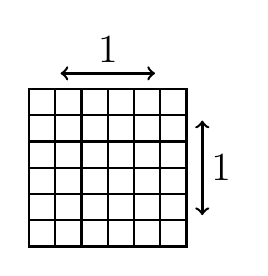
\begin{tikzpicture}[scale=2, thick]
            % Grid
            \draw[line width=1pt] (0,0) rectangle (1,1);
            \foreach \x in {1/6, 2/6, 3/6, 4/6, 5/6}
                \draw[line width=0.8pt] (\x,0) -- (\x,1);
            \foreach \y in {1/6, 2/6, 3/6, 4/6, 5/6}
                \draw[line width=0.8pt] (0,\y) -- (1,\y);
            % Horizontal arrow + 1
            \draw[<->, line width=0.9pt] (0.2,1.1) -- (0.8,1.1);
            \node at (0.5,1.25) {\Large $1$};
            % Vertical arrow + 1
            \draw[<->, line width=0.9pt] (1.1,0.2) -- (1.1,0.8);
            \node at (1.22,0.5) {\Large $1$};
        \end{tikzpicture}
        \end{center}
        mit $m$ Knoten und Gitterabstand $h=\tfrac{1}{m-1}$. Die gesamte Knotenzahl ist $n=m^2$. \\
        Die Ableitung von $f$ an der Stelle $x_0$ sei definiert durch
        \[f'(x_0) := 
        \lim_{\Delta x \rightarrow 0} \dfrac{f(x_0+\Delta x)-f(x_0)}{(x_0+\Delta x) - x_0} 
        = \lim_{\Delta x \rightarrow 0} \dfrac{f(x_0+\Delta x)-f(x_0)}{\Delta x} \]
        durch Linearisierung (Tangentengleichung) bzw. für genauere Approximationen Taylorformel ergibt sich:
        \begin{align*}
            f_L(x) &= f(x_0) + f'(x_0)(x-x_0) \\
            f(x) &= f(x_0) + f'(x_0)(x-x_0) + \tfrac{1}{2} f''(x_0)(x-x_0)^2 + \dotsc + R_n(x,x_0)
        \end{align*}
        und damit 
        \begin{align*}
            f(x+\Delta x) &= f(x_0) + f'(x_0)\Delta x + \tfrac{1}{2}f''(x_0)(\Delta x)^2 + R \tag{1}\\
            f(x-\Delta x) &= f(x_0) - f'(x_0)\Delta x + \tfrac{1}{2}f''(x_0)(\Delta x)^2 + \tilde{R} \tag{2} \\
        \end{align*}
        Mit dieser Approximation ergibt sich für die Differenzquotienten:
        \begin{align*}
            \dfrac{\diff^+}{\diff x} f(x)\mid_{x=x_0} &= \dfrac{1}{\Delta x}\left(f(x_0+\Delta x) - f(x_0)\right) 
            \tag{rechtsseitiger DQ}\\
            \dfrac{\diff^-}{\diff x} f(x)\mid_{x=x_0} &= \dfrac{1}{\Delta x}\left(f(x_0)-f(x_0+\Delta x)\right) 
            \tag{linksseitiger DQ}\\
            \dfrac{\diff}{\diff x} f(x)\mid_{x=x_0} 
            &= \dfrac{1}{2\Delta x}\left(f(x_0+\Delta x) - f(x_0-\Delta x)\right)\tag{zentraler DQ}
        \end{align*}
        Der zentrale Differenzquotienten approximiert dabei mit einer Ordnung häher als der links- und rechtsseitige 
        Differenzquotient, da quadratische Terme in (1) und (2) sich gegenseitig wegkürzen. \\ \\
        Wir nutzen dies nun um die Laplace-Operator in 2 Dimensionen zu approximieren: \\
        \begin{center}
\begin{tikzpicture}[scale=0.5, thick, every node/.style={font=\large}]

  % Gitter zeichnen
  \draw[line width=1pt] (0,0) grid (6,6);

  % Zentrum
  \def\x{3}
  \def\y{3}

  % Nachbarn markieren (blau)
  \foreach \dx/\dy in {1/0, -1/0, 0/1, 0/-1}
    \fill[mydarkblue] (\x+\dx,\y+\dy) circle (4pt);

  % Zentrumspunkt (rot)
  \fill[mydarkred] (\x,\y) circle (4pt);

  % Labels - rechts
  \node (toplabel)   [mydarkblue] at (\x+5,\y+1.5) {$(x, y{+}h)$};
  \node (centerlabel)[mydarkred]  at (\x+4.6,\y+0.5)   {$(x, y)$};
  \node (rightlabel) [mydarkblue] at (\x+5,\y-0.5) {$(x{+}h, y)$};
  % Labels - links
  \node (leftlabel)  [mydarkblue]  at (\x-5,\y-0.5)   {$(x{-}h, y)$};
  \node (bottomlabel)[mydarkblue] at (\x-5,\y-1.5) {$(x, y{-}h)$};

  % Pfeile 
  \draw[->, thick, mydarkblue] (toplabel.west)   to[out=180, in=45] (\x+0.2,\y+1+0.2);
  \draw[->, thick, mydarkred]  (centerlabel.west)to[out=180, in=45]  (\x+0.2,\y+0.2);
  \draw[->, thick, mydarkblue] (rightlabel.west) to[out=180, in=-45] (\x+1+0.2,\y-0.2);
  \draw[->, thick, mydarkblue] (leftlabel.east) to[out=0, in=-135] (\x-1-0.2,\y-0.2);
  \draw[->, thick, mydarkblue] (bottomlabel.east) to[out=0, in=-135] (\x-0.2,\y-1-0.2);

\end{tikzpicture}
        \end{center}
        Für innnere Punkte in unserem Quadratgitter gilt die sogenannte \glqq 5-Punktregel\grqq{}:
        \[-h^{-2}\left(u(x+h,y)-2u(x,y)+u(x-h,y)+u(x,y+h)-2u(x,y)+u(x,y-h)\right)=f(x,y)\]
        Durch Berücksichtigung der Randbedingung $u(x,y)=0$ für $(x,y)\in\partial Q$ ist dies äquivalent zu einem 
        linearen Gleichungssystem $Ax=b$ für den Vektor $x\in\mathbb{R}^n$ der unbekannten Knotenwerte 
        $x_i=u(P_i)$
        Die Matrix $A$ hat die Gestalt
        \[A = \left.\begin{pmatrix}
            B & -I & 0 & \dots\\
            -I & B & -I & \\
            0 & -I & B & \ddots \\
            \vdots& & \ddots & \ddots
        \end{pmatrix}\right\} n \quad \text{ mit } B = \left.\begin{pmatrix}
            4 & -1 & 0 & \dots\\
            -1 & 4 & -1 & \\
            0 & -1 & 4 & \ddots \\
            \vdots& & \ddots & \ddots
        \end{pmatrix}\right\}m\]
        und der Einheitsmatrix $I$, d.h. $B,I\in\mathbb{R}^{m\times m}$. 
        Die rechte Seite ist $b=h^2(f(P_1),\dotsc,f(P_n))^T$. \\
        Wir erhalten ein sehr großes LGS mit dünn besetzter Bandmatrix mit Bandbreite $2m+1$, symmetrisch, 
        schwach diagonaldominant, positiv definit. Es biete sich also an unsere iterativen Verfahren zum Lösen 
        anzuwenden.
    \end{egbox}
    \newpage
    \subsubsection{Konvergenzgeschwindigkeit des CG-Verfahren}
    \begin{thmbox}{Satz}[CG-Konvergenz]
        Sei $x$ die Lösung des linearen Gleichungssystems $Ax=b$. Für das CG-Verfahren gilt die Fehlerabschätzung
        \[\|x^{(k)} - x\|_A \leq 2\left(\dfrac{\sqrt{\kappa(A)-1}}{\sqrt{\kappa}}+1\right)^k \cdot \|x^{(0)}-x\|\]
        Zur Reduktion des Anfangsfehlers um den Faktor $\varepsilon$ sind circa 
        \[k(\varepsilon)\approx \tfrac{1}{2}\sqrt{\kappa(A)}\cdot \ln(\tfrac{2}{\varepsilon}) +1 \]
        Iterationsschritte erforderlich. 
    \end{thmbox}
    Für den Beweis des Satzes benötigen wir noch einen Hilfssatz:
    \begin{thmbox}{Hilfssatz}[polynomiale Normschranke]
        Für ein Polynom $p\in P_k:=\mathbb{R}_k[X]$ mit $p(0)=1$, gelte auf einer Menge $S\subset \mathbb{R}$, welche
        alle Eigenwerte von $A$ enthält, $\sup_{\mu\in S} |p(\mu)| \leq M$. Dann gilt 
        \[\|x^{(k)} - x\|_A \leq M\cdot\|x^{(0)}-x\|_A\]
    \end{thmbox}
    \textit{Beweis des Hilfssatz.} Unter Beachtung der Beziehung 
    \[\|x^{(k)}-x\|_A = \min\{\|y-x\|_A : y\in x^{(0)}+\mathcal{K}_k(A,r^{(0)})\}\]
    erhalten wir 
    \[\|x^{(k)}-x\|_A = \min_{p\in P_{k-1}}\|x^{(0)}-x+p(A)r^{(0)}\|_A\]
    Wegen $r^{(0)} = Ax^{(0)}-b = A(x^{(0)}-x)$ folgt
    \begin{align*}
        \|x^{(k)}-x\|_A &= \min_{p\in P_{k-1}} \|(I+A\cdot p(A))\cdot (x^{(0)}-x)\|_A \\
        &\leq \min_{p\in P_{k-1}} \|I+A\cdot p(A)\|_A\cdot\|x^{(0)}-x\|_A \\
        &\leq \min_{p\in P_{k-1}, p(0)=1} \|p(A)\|_A\cdot\|x^{(0)}-x\|_A 
    \end{align*}
    mit der von $A$-Norm (Energienorm)$\|\cdot\|_A$ erzeugten natürlichen Matrixnorm $\|\cdot\|_A$. \\
    Für beliebiges $y\in\mathbb{R}^n$ gilt mit einer Orthonormalbasis $\{w_1,\dotsc,w_n\}$ aus Eigenvektoren von $A$:
    \[y=\sum_{j=1}^{n}\gamma_j w_j,\quad \gamma_j = \langle y, w_j\rangle\]
    und folglich 
    \[\|p(A)y\|_A^2 = \sum_{j=1}^{n} \lambda_j p(\lambda_j)^2\gamma_j^2 
    \leq M^2 \sum_{j=1}^{n} \lambda_j \gamma_j^2 = M^2 \|y\|_A^2\]
    Dies impliziert 
    \[\|p(A)\|_A = \sup_{y\in\mathbb{R}^n\backslash\{0\}} \dfrac{\|p(A)y\|_A}{\|y\|_A}\leq M\]
    und damit die Behauptung. \qed \\ \\
    \textit{Beweis von Satz 2.21}Durch Verwendung des Hilfssatz mit $S:=[\lambda, \Lambda]$, 
    wobei $\lambda$ den kleinsten un d$\Lambda$ den größten Eigenwert von $A$ beschreibt, folgt:
    \[\|x^{(k)}-x\|_A \leq \min_{p\in P_{k-1}, p(0)=1} 
    \left(\sup_{\lambda\leq\mu\leq\Lambda}|p(\mu)|\right)\cdot\|x^{(0)}-x\|_A \]
    Dies ergibt die Behauptung wenn wir noch zeigen können, dass 
    \[\sup_{\lambda\leq\mu\leq\Lambda}|p(\mu)| 
    \leq 2\cdot \dfrac{(1-\sqrt{\tfrac{\lambda}{\Lambda}})^k}{(1+\sqrt{\tfrac{\lambda}{\Lambda}})^k}\]
    Hierbei handelt es sich um ein Problem der Bestapproximation von Polynomen bzgl. 
    der Maximumsnorm (Chebyshev-Approximation).
    Die Lösung $\overline{p}$ ist gegeben durch 
    \[\overline{p}(\mu) = \dfrac{T_k(\tfrac{\Lambda+\lambda-2\mu}{\Lambda-\lambda})}
    {T_k(\tfrac{\Lambda+\lambda}{\Lambda-\lambda})},\]
    wobei $T_k$ das $k$-te Chebyshev-Polynom auf $[-1,1]$ ist. Es folgt
    \[\sup_{\lambda\leq\mu\Lambda} = T_k\left(\dfrac{\Lambda+\lambda}{\lambda-\lambda}\right)^{-1}\]
    Aus der Darstellungen
    \[T_k(\mu) = \tfrac{1}{2}\left((\mu+\sqrt{\mu^2-1})^k+(\mu-\sqrt{\mu^2-1})^k\right), 
    \quad \text{für } \mu\in[-1,1]\]
    für die Chebyshev-Polynome folgt mittels der Identität
    \[\dfrac{\kappa+1}{\kappa-1} + \sqrt{\left(\dfrac{\kappa+1}{\kappa-1}\right)^2-1} 
    = \dfrac{\kappa+1}{\kappa-1} + \dfrac{2\sqrt{\kappa}}{\kappa-1} = \dfrac{(\sqrt{\kappa}+1)^2}{\kappa - 1}
    = \dfrac{\sqrt{\kappa}+1}{\sqrt{\kappa}-1}\]
    die folgende Abschätzung nach unten:
    \[T_k\left(\dfrac{\Lambda+\lambda}{\Lambda-\lambda}\right) = T_k\left(\dfrac{\kappa+1}{\kappa-1}\right)
    = \dfrac{1}{2}\left(\left(\dfrac{\sqrt{\kappa}+1}{\sqrt{\kappa}-1}\right)^k + 
    \left(\dfrac{\sqrt{\kappa}-1}{\sqrt{\kappa}+1}\right)^k\right) 
    \geq \left(\dfrac{\sqrt{\kappa}+1}{\sqrt{\kappa}-1}\right)^k\]
    Also wird $\sup_{\lambda\leq\mu\leq\Lambda}\overline{p}(\mu)
    \leq 2\left(\tfrac{\sqrt{\kappa}-1}{\sqrt{\kappa}-1}\right)^k$, was die erste Ungleichung des Satzes zeigt. \\
    Für den zweiten Teil betrachten wir die Anzahl der Schritte, dass
    \[2\left(\dfrac{\sqrt{\kappa}-1}{\sqrt{\kappa}-1}\right)^{k(\varepsilon)} < \varepsilon \quad \iff \quad 
    k(\varepsilon) > \ln(\tfrac{2}{\varepsilon})\cdot
    \left(\ln\left(\dfrac{\sqrt{\kappa}-1}{\sqrt{\kappa}-1}\right)\right)^{-1}\]
    Wegen der Reihendarstellung $\ln\tfrac{x+1}{x-1} = 2(\tfrac{1}{x} + \tfrac{1}{3}\tfrac{1}{x^3} 
    + \tfrac{1}{5}\tfrac{1}{x^5} + \dotsc)$ ist die zweite Ungleichung genau dann erfüllt wenn 
    \[k(\varepsilon) > \tfrac{1}{2}\sqrt{\kappa}\ln(\tfrac{2}{\varepsilon})\]
    \qed
% !TeX root = ../script.tex
\section{Eigenwertprobleme}
\subsection{Einleitung}
Aus der linearen Algebra ist das klassische Eigenwertproblem bekannt. Gegeben sei eine Matrix 
$A\in\mathbb{K}^{n\times n}$ und gesucht sind $\lambda\in\mathbb{K}$ und $v\in\mathbb{K}^n$, $v\neq 0$ 
sodass $Av=\lambda v$. Das Umstellen des Eigenwertproblems ergibt das System $(A-\lambda I)v=0$ (*). Hierbei muss 
$A-\lambda I$ singulär sein, sonst ist die einedeuige Lösung des Systems gegeben durch $v=0$.\\
Per Hand würden wir hier nun das charakteristische Poylnom $\chi_A(\lambda)=\det(A-\lambda I)$ aufstellen und 
dessen Nullstellen bestimmen, da dies genau die Werte für $\lambda$ sind, für welche das obige System nicht-triviale
Lösungen hat. \\
Für die nuerische Berechung der Eigenwerte ist dies nicht ratsam, da Nullstellenbestimmung bei Polynomen 
hochgradig schlecht konditioniert ist. \\
Wir stellen folgende Zusammenhänge der Berechnung von Eigenwerten und Eigenvektoren fest:
\begin{enumerate}
    \item[a)] Eigenwert-Bestimmung: Eigenvektor über LGS (*).
    \item[b)] Eigenvektor-Bestimmung: 
        Eigenwert über Rayleigh-Quotient $\lambda=\dfrac{\langle Av,v\rangle}{\|v\|_2^2}$ 
\end{enumerate}
\subsection{Einschließungssätze und Stabilität}
\begin{thmbox}{Hilfssatz}
    Seien $A,B\in\mathbb{K}^{n\times n}$ beliebige Matrizen und $\|\cdot\|$ eine natürliche Matrixnorm. Dann gilt 
    für jeden Eigenwert $\lambda$ von $A$, welcher nicht zugleich auch Eigenwert von $B$ ist, die Beziehung
    \[\|(\lambda I-B)^{-1}(A-B)\|\geq 1\]
\end{thmbox}
\textit{Beweis.} Ist $w$ ein Eigenwektor vom Eigenwert $\lambda$ von $A$, so folgt aus der Identität 
$(A-B)w = (I\lambda - B)w$, dass wenn $\lambda$ kein Eigenwert von $B$ ist, d.h. $\lambda I-B$ invertierbar: 
\[(\lambda I-B)^{-1}(A-B)w=w\]
Demnach ist also 
\[1\leq \sup_{x\in\mathbb{K}^n\backslash\{0\}} \dfrac{\|(\lambda I-B)^{-1}(A-B)x\|}{\|x\|}
=\|(\lambda I-B)^{-1}(A-B)\|\]
\subsubsection{Gerschgorin-Kreise}
\begin{thmbox}{Satz}[Satz von Gerschgorin]
    Alle Eigenwerte eine Matrix $A\in\mathbb{K}^{n\times n}$ liegen in der Vereinigung der sogenannten 
    Gerschgorin-Kreise
    \[K_j := \left\{z\in\mathbb{C} : |z-a_{jj}|\leq \sum_{k\neq j} |a_{jk}|\right\},
    \qquad \text{für } j=1,\dotsc,n.\]
    Für eine Teilmenge $I\subset\{1,\dotsc,n\}$ gilt, sind die Mengen $U=\displaystyle \bigcup_{j\in I} K_j$ 
    und $V=\displaystyle \bigcup_{j\notin I} K_j$ disjunkt, so liegen in $U$ genau $m:=|I|$ und in $V$ genau $n-m$ 
    Eigenwerte von $A$ (mehrfache Eigenwerte werden entsprechend ihrer algebraischen Vielfachheit gezählt).
\end{thmbox}
\textit{Beweis.} Zur ersten Behauptung: Wir setzen $B=diag(a_{jj})$ in dem Hilfssatz 3.1 und nehmen 
$\|\cdot\|_\infty$ als natürliche Matrixnorm. Für $\lambda\neq a_{jj}$ folgt dann 
\[\|(\lambda I -D)^{-1}(A-D)\|_\infty = \max_{j=1,\dotsc,n}\dfrac{1}{\lambda-a_{jj}}\sum_{k\neq j} |a_{jk}|\geq 1,\]
d.h. $\lambda$ liegt in einem der Gerschgorin-Kreise. \\
Für den zweiten Teil sei o.B.d.A. $I=\{1,\dotsc,m\}$. \\
Setzen wir $A_t = D + t(A-D)$, dann liegen genau $m$ Eigenwerte von $A_0=D$ in $U$ und $n-m$ 
Eigenwerte in $V$. Das selbe folgt auch für $A_1=A$, da die Eigenwerte von $A_t$ stetige Funktionen in $t$ sind. 
\qed \\ \\
Ein Alternativer Beweis zur ersten Behauptung liefert eine Betrachtung des 
Eigenwertproblems $Ax=\lambda x$ mit $x\neq 0$. Offensichtlich existiert ein $x_i$ mit $|x_j|\leq |x_i|$ für alle 
$j\neq i$. Die $i$-te Komponente von $Ax$ ist gegeben durch 
\[\lambda x_i = (Ax)_i = \sum_{j=1}^{m} a_{jj}x_j \]
Somit folgt 
\[|\lambda-a_{ii}| = \left|\sum_{j\neq i} a_{ij} \dfrac{x_j}{x_i}\right|\leq \sum_{j\neq i}|a_{ij}|\]
Demnach liegt $\lambda\in K_i$.\qed
\begin{egbox}
    Gegeben sei die Matrix 
    \[A = \begin{pmatrix}
        1 & 0.1 & -0.2 \\ 0 & 2 & 0.4 \\ -0.2 & 0 & 3
    \end{pmatrix}\]
    Es ergeben sich die folgenden Gerschgori-Kreise:
    \begin{align*}
        K_1 = \{z\in\mathbb{C} : |z-1|\leq 0.3\} \\
        K_2 = \{z\in\mathbb{C} : |z-2|\leq 0.4\} \\
        K_3 = \{z\in\mathbb{C} : |z-3|\leq 0.2\} \\
    \end{align*}
    \begin{center}
        \begin{tikzpicture}[scale=3]
        % Axes
        \draw[->] (-0.2,0) -- (4,0) node[right] {Re\((z)\)};
        \draw[->] (0,-1) -- (0,1) node[above] {Im\((z)\)};
        
        % Circle 1
        \draw[thick] (1,0) circle (0.3);
        \filldraw (1,0) circle (0.02) node[below] {\(1\)};
        \draw[thick] (1,0) -- ++(70:0.3);
        \node at ($(1,0)+(70:0.4)$) {\(r = 0.3\)};
        
        % Circle 2
        \draw[thick] (2,0) circle (0.4);
        \filldraw (2,0) circle (0.02) node[below] {\(2\)};
        \draw[thick] (2,0) -- ++(70:0.4);
        \node at ($(2,0)+(70:0.5)$) {\(r = 0.4\)};
        
        % Circle 3
        \draw[thick] (3,0) circle (0.2);
        \filldraw (3,0) circle (0.02) node[below] {\(3\)};
        \draw[thick] (3,0) -- ++(70:0.2);
        \node at ($(3,0)+(70:0.3)$) {\(r = 0.2\)};

        \end{tikzpicture}
    \end{center}
\end{egbox}
\newpage
\subsubsection{Stabilität von Eigenwerten}
\begin{thmbox}{Satz}[Stabilitätssatz]
    Sei $A\in\mathbb{K}^{n\times n}$ eine Matrix, zu der es $n$ linear unabhängige Eigenvektoren gibt 
    $\{w^{(1)},\dotsc,w^{(n)}\}$ und sei $B\in\mathbb{K}^{n\times n}$ eine zweite Matrix. Dann gibt es zu 
    jedem Eigenwert$\lambda(B)$ von $B$ einen Eigenwert $\lambda(A)$ von $A$, sodass mit der Matrix 
    $W=(w^{(1)}|\dotsc|w^{(n)})$ gilt
    \[|\lambda(A)-\lambda(B)|\leq\Cond_2(W)\cdot\|A-B\|_2\]
\end{thmbox}
\textit{Bewies.} Die Eigenwertgleichungen $Aw^{(i)}=\lambda_i(A)w^{(i)}$ lassen sich in der Form 
$AW=W\cdot\diag(\lambda_i(A))$ schreiben, d.h. $A=W\cdot\diag(\lambda_i(A))\cdot W^{-1}$ ist ähnlich zu der 
Diagonalmatrix $\Lambda = \diag(\lambda_i(A))$. Wenn nun $\lambda=\lambda(B)$ kein Eigenwert von $A$ ist, so gilt 
\[\|(\lambda I - A)^{-1}\|_2 = \|W(\lambda I - \Lambda)^{-1}W^{-1}\|_2 
\leq \|W\|_2\cdot\|W^{-1}\|_2\cdot\|(\lambda I-\Lambda)^{-1}\| 
= \Cond_2(W)\cdot \max_{i=1,\dotsc,n} |\lambda-\lambda_i(A)|^{-1}\]
Mit dem Hilfssatz 3.1 folgt dann die Behauptung. \qed \\ \\
Für hermitische Matrizen $A\in\mathbb{K}^{n\times n}$ existiert bekannterweise eine Orthonormalbasis des 
$\mathbb{K}^{n\times n}$ aus Eigenvektoren, sodass die Matrix $W$ als unität angenommen werden kann, 
d.h. $ww^{-*}=I$. In diesem Fall gilt $\Cond_2(W)=\|W^{-*}\|_2\cdot\|W\|_2 = 1$. \\ \\
\textbf{Regel:} Allgemein kann man sagen, dass das Eigenwertproblem für hermtische Matrizen gut konditioniert
ist, während das allgemeine Eigenwertproblem je nach Größe von $\Cond_2(W)$ beliebig schlecht konditioniert 
sein kann.
\subsection{Iterative Verfahren}
Im folgenden wollen wir ein iteratives Verfahren zu Lösung des partiellen Eigenwertproblems einer 
Matrix $A\in\mathbb{K}^{n\times n}$ betrachten.
\subsubsection{Potenz-Methode}
\begin{defbox}
    Die Potenzmethode (Von-Mises-Iteration) erzeugt ausgehend von einem Startvektor $z^{(0)}\in\mathbb{C}^n$ mit
    $\|z^0\|=1$ eine Folge von Iterationen $z^{(t)}\in\mathbb{C}^n, t=1,2,\dotsc$ durch 
    \[\tilde{z}^{(t)}=Az^{(t-1)} \quad\text{und}\quad z^{(t)} = \tfrac{\tilde{z}^{(t)}}{\|\tilde{z}^{(t)}\|}.\]
    Für einen beliebigen  Index $k\in\{1,\dotsc,n\}$, (z.B. maximale Komponente von $z^k$) wird gesetzt:
    \[\lambda^{(t)} = \dfrac{(Az^{(t)})_k}{(z^{(t)})_k}\]
    \textit{Zur Normierung wird üblicherweise $\|\cdot\|=\|\cdot\|_2$ oder $\|\cdot\|_\infty$ verwendet.} 
\end{defbox}
Zur Analyse des Verfahrens nehmen wir an, dass die Matrix $A$ diagonalisierbar ist, d.h. ähnlich zu einer 
Diagonalmatrix ist. Dies ist äquivalent zu der Tatsache, dass $A$ eine Basis von Eigenvektoren 
$\{w^{(1)},\dotsc,w^{(n)}\}$ besitzt. Weiter seien diese Eigenvektoren $w^{(i)}$ normiert. \\
Wir nehmen an, dass $z^{(0)}$ eine nicht-triviale Komponente bezüglich $w^{(n)}$ besitzt. 
(Dies ist keine wesentliche Einschränkung, da aufgrund des unvermeidbaren Rundungsfhlers dieser Fall der 
Iteration sicher einmal auftritt)
\newpage
\begin{thmbox}{Satz}[Potenz-Methode]
    Die Matrix $A$ sei diagonalisierbar und ihr betragsgrößter Eigenwert sei separiert von den anderen 
    Eigenwerten, d.h. $|\lambda_n|>|\lambda_{n-1}|\geq|\lambda_{n-2}|\geq\dotsc\geq|\lambda_1|$. \\ 
    Der Startvektor $z^{(0)}$ habe eine nicht-triviale Komponente bezüglich des zugehörigen Eigenvektors $w^{(n)}$.
    Dann gibt es Zahlen $\delta_t\in\mathbb{C}, |\delta_t|=1$, 
    sodass $\|z^{(t)}-\delta_t\cdot w^{(n)}\|\rightarrow 0$ für $t\rightarrow\infty$ und es gilt
    \[\lambda^{(t)}-\lambda_n = \mathcal{O}\left(\left|\dfrac{\lambda_{n-1}}{\lambda_n}\right|^t\right)\qquad 
    \text{ für } t\rightarrow \infty\]
\end{thmbox}
\textit{Beweis.} Sei $z^{(0)}=\sum_i \alpha_i\cdot w^{(i)}$ die Basisdarstellung des Startvektors 
(mit $\alpha_n\neq 0$). Für die Iterierten gilt:
\[z^{(t)} = \dfrac{\tilde{z}^{(t)}}{\|\tilde{z}^{(t-1)}\|} = \dfrac{Az^{(t-1)}}{\|Az^{(t-1)}\|} 
= \dotsc = \dfrac{A^tz^{(0)}}{\|A^tz^{(0)}\|}\]
Dabei gilt:
\[A^tz^{(0)} = \sum_{i=1}^{n}\alpha_i\lambda_i^tw^{(i)} = \lambda_n^t \alpha_n\cdot\left(w^{(n)} + 
\sum_{i\neq n} \dfrac{\alpha_i}{\alpha_n}\left(\dfrac{\lambda_i}{\lambda_n}\right)^t w^{(i)}\right)\]
Wegen $|\tfrac{\lambda_i}{\lambda_n}|\leq \rho:=|\tfrac{\lambda_{n-1}}{\lambda_n}|<1$ für $i=1,\dotsc,n-1$ folgt
\[A^tz^{(0)} = \lambda_n^t\alpha_n(w^{(n)}+\mathcal{O}(\rho^t))
\qquad \text{ für } t\rightarrow \infty\]
Dies ergibt:
\[z^{(t)} = \dfrac{\lambda_n^t\alpha_n(w^{(n)}+
\mathcal{O}(1))}{|\lambda_n^t\alpha_n|\cdot\|w^{(n)}+\mathcal{O}(\rho^t)\|}
= \underbrace{\dfrac{\lambda_n^t\alpha_n}{|\lambda_n^t\alpha_n|}}_{=:\delta_k}\cdot (w^{(n)}+\mathcal{O}(\rho^t))\]
Dabei ist $\delta_t\in\mathbb{C}$ und $|\delta_t|=1$, daher folgt die erste Aussage.\\
Weiter gilt 
\begin{align*}
    \lambda^{(t)} &= \dfrac{(Az^{(t)})_k}{(z^{(t)})_k} \\
    &= \dfrac{(A^{t+1}z^{(0)})_k}{\|(A^{t+1}z^{(0)})_k\|}\cdot\dfrac{{\|(A^{t+1}z^{(0)})_k\|}}{(A^tz^{(0)})_k} \\
    &= \dfrac{\lambda_n^{t+1}(\alpha_n w_{n,k}+\sum_{i\neq n} \alpha_i(\tfrac{\lambda_i}{\lambda_n})^{t+1}w_{i,k})}
    {\lambda_n^t(\alpha_n w_{n,k}+\sum_{i\neq n} \alpha_i(\tfrac{\lambda_i}{\lambda_n})^tw_{i,k})} \\
    &= \lambda_n + \mathcal{O}\left(\left|\dfrac{\lambda_{n-1}}{\lambda_n}\right|^t\right)\qquad 
    \text{ für } t\rightarrow \infty
\end{align*}
\qed \\ \\
Die Konvergenz der Potenzmethode ist umso besser, je mehr der betragsgrößte Eigenwert $\lambda_n$ von den übrigen 
betragsmäßig separiert ist. Der Beweis ist verallgemeinerbar für betragsgrößte Eigenwerte, welche merhfach 
auftreten, sofern die Matrix diagonalisierbar ist. \\ \\
\subsubsection{Inverse Iteration} 
Als nächstes wollen wir uns die \glqq{}Inverse Iteration\grqq{} nach
Wielandt anschauen. \\
Wir nehmen an, man hat bereits eine Näherung $\tilde{\lambda}$ für einen Eigenwert $\lambda_k$ der regulären Matrix 
$A$ (z.B. durch Einschließungssätze). Die Näherung sei gut in dem Sinne, 
dass $|\lambda_k-\tilde{\lambda}|\ll |\lambda_i-\tilde{\lambda}|$ für $i\neq k$.\\
Sei $\lambda$ ein Eigenwert von $A$, dann ist $\lambda^{-1}$ ein Eigenwert von $A^{-1}$. 
Wir betrachten das Eigenwertproblem, welches sich für die Matrix $A-\tilde{\lambda}I$ ergibt:
\[(A-\tilde{\lambda}I)v=\xi v \iff (A-\tilde{\lambda}I-\xi I)v = 0 \iff (A-(\tilde{\lambda}+\xi)I)v=0\]
Also ist $\xi=\lambda_k-\tilde{\lambda}$ ein Eigenwert von $A-\tilde{\lambda}I$ und folglich ist 
$\mu=\tfrac{1}{\xi}=(\lambda_k-\tilde{\lambda})^{-1}$ ein Eigenwert von $(A-\tilde{\lambda}I)^{-1}$. \\
Allgemeiner hat im Falle $\tilde{\lambda}\neq\lambda_k$ die Matrix $(A-\tilde{\lambda}I)^{-1}$ die Eigenwerte 
$\mu_i = (\lambda_i-\tilde{\lambda})^{-1}$ für $i=1,\dotsc,n$ un des gilt 
\[\left|\dfrac{1}{\lambda_k-\tilde{\lambda}}\right| \gg \left|\dfrac{1}{\lambda_i-\tilde{\lambda}}\right|\qquad 
\text{für } i\neq k\]
\begin{defbox}
    Die inverse Iteration besteht in der Anwendung der Potenzmethode auf die Matrix $(A-\tilde{\lambda}I)^{-1}$
    mit einer a priori Schätzung $\tilde{\lambda}$ zum gesuchten Eigenwert $\lambda_k$. \\ 
    Ausgehend von einem Startwert $z^{(0)}$ werden Iterierte $z^{(t)}$ bestimmt als Lsg. der Gleichungssysteme
    \[(A-\tilde{\lambda}I)z^{(t)} = \tilde{z}^{(t-1)},
    \qquad z^{(t)} = \dfrac{\tilde{z}^{(t)}}{\|\tilde{z}^{(t)}\|}\]
    Die zugehörige Eigenwertnäherung wird bestimmt durch 
    \[\mu^{(t)}=\dfrac{(z^{(t)})_k}{((A-\tilde{\lambda}I)z^{(t)})_k}\]
    mit Nenner $\neq 0$ (oder im symmetrischen Fall mit Hilfe der Rayleigh-Quotienten).
\end{defbox}
Aufgrund der Aussagen über Potenzmethoden liefert die inverse Iteration also für eine diagonalisierbare Matrix
jeden Eigenwert, zu dem bereits eien hinreichend gute Näherung bekannt ist.
\subsection{Page-Rank-Algorithmus}
Das Ziel des Page-Rank-Algorithmus ist die Bestimmung der Ausgabereihenfolge bei Suchergebnissen. Dabei berufen 
wir uns auf folgende Regeln:
\begin{enumerate}
    \item[(1)] Eine Website erhält eine umso höhere Bewertung, je mehr Links auf sie zeigen.
    \item[(2)] Links von höher bewerteten Websites soll relevanter sein, als solceh von unbedeutenden
    \item[(3)] Ein Link von einer Website, die wenig Links nach außen hat, soll höher gewichtet werden als der
        von einer Website mit vielen Links nach außen. 
\end{enumerate}
Wir beschreiben unser Model als ein Netz mit $n$ Seiten, wobei ein Index $k$ immer für eine Seite steht. \\
Gesucht ist die Bedeutung einer Seite $x_k\in\mathbb{R}$ \\
$L_k$ sei die Menge der Seiten, die auf $k$ verlinken, Links auf Seiten von sich selbst werden dabei nicht
berücksichtigt. \\
$n_k$ sei die Anzahl der Links, der Webite $k$ nach außen.\\
Wir modellieren mittels folgendem LGS
\[x_k = \sum_{j\in L_k}\tfrac{1}{n_j}\cdot x_j\]
Die Gleichung $x=Ax$ entspricht hierbei der Eigenwertgleichung für den Eigenwert $\lambda=1$. \\
Der historische Ansatz von Google ist die Potenzmethode:
\[x = \begin{pmatrix}
    x_1 \\ \vdots \\ x_n
\end{pmatrix}, \qquad A_{ij} = a_{ij} = \begin{cases}
    \tfrac{1}{n_j}, & \text{falls die Seite } j \text{ auf die Seite } i \text{ verlinkt} \\
    0, & \text{sonst}
\end{cases}\]
\newpage
\subsubsection{Stochastische Vektoren/Matrizen}
\begin{defbox}
    Ein Vektor $p\in\mathbb{R}^n$ heißt stochastischer Vektor, wenn alle Elemente $p_i$ nicht-negativ sind und die 
    Summe der Elemente des Vektors gleich 1 ist, d.h. $\sum_{i} p_i = 1$. \\
    Eine Matrix $A\in\mathbb{R}^{n\times n}$ heißt stochastische Matrix, wenn ale Spalten der Matrix stochastische 
    Vektoren sind, d.h.
    \[a_{ij}\geq 0\ \forall i,j \quad \text{und } \quad \sum_{i=1}^n a_{ij}=1\ \forall j\]
\end{defbox}
\begin{thmbox}{Lemma}
    Sei $A\in\mathbb{R}^{n\times n}$ eine stoch. Matrix und $p\in\mathbb{R}^{n}$ ein stoch. Vektor, dann ist 
    das Produkt $Ap\in\mathbb{R}^{n\times n}$ wieder ein stoch. Vektor.
\end{thmbox}
\textit{Beweis.} Es sei $a_i$ die $i$-te Spalte der Matrix $a_i$, d.h. $a_i$ ist ein stoch. Vektor
\begin{align*}
    A\cdot p = A\cdot \begin{pmatrix}
    p_1 \\ \vdots \\ p_n
\end{pmatrix} &= p_1\cdot a_1 + \dotsc + p_n\cdot a_n \\
&= \sum_{i} (p_1a_{i1} + \dotsc + p_na_{in}) \\
&= p_1\sum_{i}a_{i1} + \dotsc +  p_n\sum_{i}a_{in} \\
&= p_1\cdot 1 + \dotsc + p_n\cdot n = 1
\end{align*}
Weiter gilt offensichtlich $(Ap)_{ij}\geq 0$.\qed
\begin{thmbox}{Lemma}
    Seien $A,B\in\mathbb{R}^{n\times n}$ stoch. Matrizen, dann ist das Produkt $A\cdot B$ wieder eine stoch. Matrix.
\end{thmbox}
\textit{Beweis.} Folgt direkt aus Lemma 3.9.
\begin{thmbox}{Satz}
    Eine stochastische Matrix $A$ hat immer den Eigenwert $1$. Der Betrag aller anderen Eigenwerte ist
     kleiner oder gleich 1.
\end{thmbox}
\textit{Beweis.} Für den ersten Teil nutzen wir aus, dass $A$ und $A^T$ die gleichen Eigenwerte, da $A$ und $A^T$ die 
gleiche Determinante besitzten und damit die charakteristischen Polynome $\chi_A(\lambda) = \det(A-\lambda I) 
= \det(A^T-\lambda I) = \chi_{A^T}(\lambda)$. \\
Weiter ist die Summe der Elemente jedes Zeilenvektors von $A^T$ ist gleich 1 (da $A$ stoch.), 
somit ist $e=(1,\dotsc,1)^T$ ein Eigenvektor von $A^T$ mit Eigenwert $1$. Somit besitzt auch die Matrix $A$ den 
Eigenwert $\lambda = 1$. \\
Angenommen es existiert ein Eigenvektor $v$ zum Eigenwert $\lambda$ mit $|\lambda|>1$, dann gilt
\[A^n v = A^{n-1}(Av) = A^{n-1}\lambda v = \lambda A^{n-1}v = \dotsc = \lambda^n v\]
Für die Länge dieses Vektors gilt $\|\lambda^n v\| = |\lambda^n|\cdot \|v\|$ ein exponentieller Wachstum in $n$, da 
$|\lambda|>1$. \\
Daraus folgt, dass für große $n$ ein Element $(A^n)_{ij}$ exisitert, welches größer als $1$ ist.\\
Da nach Lemma 3.10 die Matrix $A^n$ stoch. ist bildet dies einen Widerspruch.\qed
\begin{thmbox}{Lemma}
    Die Bewertungsmatrix $A$ des Page-Rank-Algorithmus ist eine stoch. Matrix.
\end{thmbox}
\textit{Beweis.} Offensichtlich gilt $a_{ij}\geq 0$, weiter gilt
\[\sum_{i=1}^n a_{ij} = n_j\cdot \dfrac{1}{n_j} + (n-n_j)\cdot 0 = 1\]
\qed
\begin{egbox}
    Wir betrachten ein einfaches Netz mit $4$ Knoten:  \\
    \begin{center}
        \begin{tikzpicture}[>=Stealth, node distance=2.5cm, every node/.style={circle, draw, minimum size=1cm}, auto]

        % Knoten
        \node (1) at (0,2.5) {1};
        \node (2) at (0,0) {2};
        \node (3) at (2.5,2.5) {3};
        \node (4) at (2.5,0) {4};

        % Kanten
        \draw[->, bend left=15] (1) to (3);
        \draw[->, bend left=15] (3) to (1); 
        \draw[->, bend left=15] (1) to (4); 
        \draw[->, bend left=15] (4) to (1); 
        \draw[->] (1) -- (2);
        \draw[->] (2) -- (4);
        \draw[->] (4) -- (3);
        \draw[->] (2) -- (3);

        \end{tikzpicture}
    \end{center}
    Es ergibt sich folgendes Gleichungssystem:
    \[\begin{pmatrix}
        x_1\\ x_2\\ x_3\\ x_4
    \end{pmatrix} = \begin{pmatrix}
        0 & 0 & 1 & 1/2 \\ 
        1/3 & 0 & 0 & 0 \\
        1/3 & 1/2 & 0 & 1/2 \\
        1/3 & 1/2 & 0 & 0
    \end{pmatrix}\cdot \begin{pmatrix}
        x_1\\ x_2\\ x_3\\ x_4
    \end{pmatrix}\]
    Lösen dieses linearen Gleichungssystems liefert:
    \[x \in \text{span}\left\{\begin{pmatrix}
        0.72 \\ 0.24 \\ 0.54 \\ 0.36
    \end{pmatrix}\right\}\]
    Demnach hat die erste Website die höchste Bewertung.
\end{egbox}
% !TeX root = ../script.tex

\section{Krylov-Raum-Methoden für EW-Probleme}
Wir verfolgen die gleiche Idee, wie auch schon bei linearen Gleichungssystemen, d.h. die ursprünglich hochdimensionalen
Probleme, werden durch geeignete Unterräume (Krylov-Räume) in kleinere Probleme umgewandelt. \\
Wir erhalten dabei ein iteratives Vorgehen, zu betrachtende Beispiele sind die Arnoldi-Methode und die 
Lanczos-Methode.

Wir betrachten also die Eigenwertgleichung $Az=\lambda z$ mit $A\in\C^{n\times n}$ 
(ab jetzt erlauben wir auch komplexe Matrizen), wobei $A$ eine sehr große
Matrix ist, typischerweise $n\geq 10^4$.

\subsection{Galerkin-Approximation}
Eigenwertprobleme können äquivalent in Variationsform (schwache Formulierung) geschrieben werden, diese besagt: \\
$z\in\C^n$ ist genau dann ein Eigenvektor von $A$ zum Eigenwert $\lambda\in\C$, wenn
%
\begin{align*}
  \langle Az,y\rangle_2 
  = \lambda\langle z,y\rangle_2 \quad\forall\,y\in\C^n 
  \tag{1}\label{eq:galerkinEQ1}
\end{align*}
%
Diese Äquivalenz gilt, da aus $\langle r, y\rangle_2 = 0$ für alle $y\in\C^{n}$ folgt, dass $r=0$ sein muss, 
in unserem Fall ist $r=Az-\lambda z$ das Residuum des Eigenwertproblems.

Sei $K_m=\Span\{q^{(1)},\dots,q^{(m)}\}$ ein geeignet gewählter Unterraum von $\C^n$ kleiner Dimension, d.h. 
$\dim K_m=m\ll n$, dann wird das $n$-dimensionale Eigenwertproblem (\ref{eq:galerkinEQ1}) mit 
folgendem $m$-dimensionalem Eigenwertproblem approximiert: 
%
\begin{align*}
  \text{suche } z\in K_m, \ \lambda\in\C : 
  \quad \text{mit}\quad 
  \langle Az,y\rangle_2 
  = \lambda\langle z,y\rangle_2 
  \quad\forall\,y\in K_m
\end{align*}
%
Aufgrund der Bilinearität des Skalarproduktes reicht es auch, wenn wir nur die erzeugenden $q^{(i)}$ betrachten, 
statt alle $y\in K_m$. 

Wir entwickeln die Eigenvektoren $z\in K_m$ bzgl. der gegebenen Basis:
%
\begin{align*}
  z = \sum_{j=1}^{m} \alpha_j q^{(j)}
\end{align*}
%
und erhalten somit das Galerkin-System
%
\begin{align*}
  \sum_{j=1}^{k} \alpha_j \langle Aq^{(j)},q^{(i)}\rangle_2 
  = \lambda\cdot\sum_{j=1}^{k} \alpha_j \langle q^{(j)},q^{(i)}\rangle_2
  \qquad\forall\,i=1,\dots,m
\end{align*}
Dabei charakterisieren die $\alpha_i$ unser gesuchtes $z$, wir schreiben dieses System daher typischerweise 
in kompakter Form als Eigenwertproblem
%
\begin{align*}
  \mathcal{A}\alpha = \lambda\mathcal{M}\alpha
\end{align*} 
%
mit Vektoren $\alpha=(\alpha_1,\dots,\alpha_m)$ und Matrizen
$\mathcal{A}=(\langle Aq^{(j)}, q^{(i)}\rangle_2)_{i,j=1}^m$, 
$\mathcal{M} = (\langle q^{(j)}, q^{(i)}\rangle_2)_{i,j=1}^m$.

Im Folgenden betrachten wir immer die \textit{kartesische Repräsentation} der Basisvektoren $q^{(i)}=(q_j^{(i)})_{j=1}^n$ 
und somit schreibt man das Galerkin-EW-Problem in der Form\footnote{
  Als Erinnerung: Im Komplexen ist das Standardskalarprodukt definiert durch 
  $\langle x,y\rangle_2 = \sum_i \overline{x}_i\cdot y_i$
}
%
\begin{align*}
  \sum_{j=1}^{m} \alpha_j\cdot \sum_{k,l=1}^{n} a_{k,l}\cdot \overline{q_k}^{(j)}\cdot q^{(i)}_l 
  = \lambda\cdot \sum_{j=1}^{m} \alpha_j \cdot\sum_{k,l=1}^{n}\overline{q_k}^{(j)}\cdot q^{(i)}_l
  \quad\forall\, i=1,\dots,m
\end{align*}
%
Mit $\mathcal{Q}^{(m)}=[q^{(1)},\dots,q^{(m)}]\in\C^{n\times m}$ kann dies in kompakter Form
%
\begin{align*}
  \mathcal{Q}^{(m)H}A\mathcal{Q}^{(m)}\alpha = \lambda \mathcal{Q}^{(m)H}\mathcal{Q}^{(m)}\alpha
\end{align*}
formuliert werden.

Wenn $\{q^{(1)},\dots,q^{(m)}\}$ eine Orthonormalbasis von $K_m$ ist, reduziert sich dies zum normalen EW-Problem:
%
\begin{align*}
  \underbrace{\mathcal{Q}^{(m)H}A\mathcal{Q}^{(m)}}_{=: H^{(m)}\in\C^{m\times m}}\alpha 
  = \lambda \alpha 
  \tag{2}\label{eq:galerkinEQ2}
\end{align*}
%
Falls $H^{(m)}$ eine spezielle Struktur hat (z.\,B. Hessenberg-Matrix oder symmetrische Tridiagonalgestalt), dann kann 
das EW-Problem mit niedriger Dimension (\ref{eq:galerkinEQ2}) mit z.B. QR-Methode gelöst werden. 

Seine Eigenwerte, genannt \textit{Ritz-Eigenwerte}, können als Approximationen der dominanten Eigenwerte der 
ursprünglichen Matrix $A$ betrachtet werden. 

\begin{colbox}{Bemerkung}[Krylov-Methode] 
  \begin{enumerate}
    \item[1.] Wähle geeignete Unterräume $K_m\in\C  ^{m\times m}$, $m\ll n$ (Krylov-Räume) durch Verwendung der 
    Matrix $A$ und deren Potenz.
    \item[2.] Konstruiere eine Orthonormalbasis $\{q^{(1)},\dots, q^{(m)}\}$ von $K_m$ mit der stabilisierten 
    Version des Gram-Schmidt-Algorithmus und setze $\mathcal{Q}^{(m)}:=[q^{(1)},\dots,q^{(m)}]$.
    \item[3.] Berechne die Matrix $H^{(m)}:=\mathcal{Q}^{(m)H}A\mathcal{Q}^{(m)}$, welche 
    konstruktionsbedingt eine Hessenberg-Matrix oder im hermiteschen Fall eine hermitesche Tridiagonalmatrix ist. 
    \item[4.] Löse das Eigenwertproblem der reduzierten Matrix $H^{(m)}\in\C^{m\times m}$ durch die 
    QR-Methode.
    \item[5.] Die Eigenwerte von $H^{(m)}$ als Näherung der dominanten (betragsgrößten) Eigenwerte 
    von $A$. Im Falle des betragskleinsten Eigenwert, muss die Matrix $A^{-1}$ betrachtet werden (Konstruktion 
    der Unterräume $K_m$ kann sehr aufwendig sein).
  \end{enumerate}
\end{colbox}

\subsection{Arnoldi-Methode}
\textbf{Idee:} \\
Die Potenzmethode verwendet nur die aktuelle Iterierte $A^mq$ mit $m\ll n$ für den normierten Startvektor 
$q\in\C^n$ mit $\vertn{2}{q}_2=1$, ignoriert aber die bereits berechneten Iterierten $\{q,Aq,A^2q,\dots,A^{m-1}q\}$.

Wir wollen diese bereits bestimmten Informationen nun nutzen und erstellen eine sogenannte \textit{Krylov-Matrix}:
%
\begin{align*}
  K_m = [q,Aq,A^2q,\dots,A^{m-1}q]
  \quad\text{mit }1\leq m\leq n
\end{align*}
%
Die Spalten dieser Matrix sind jedoch nicht orthogonal zueinander, außerdem konvergiert $A^tq$ gegen den 
Eigenvektor zum betragsgrößten Eigenwert, d.h. $K_m$ ist schlecht konditioniert\footnote{
  Für nicht-invertierbare Matrizen $A\in\C^{n\times m}$ ist die Konditionszahl über das Pseudoinverse definiert
}, da sich die letzten Spalten kaum ändern. 

Wie wir sehen werden, ist die Konstruktion in eine orthogonale Basis mit dem Gram-Schmidt-Algorithmus instabil, 
wir wählen daher als Alternative in der Arnoldi-Methode die Verwendung einer stabilisierten Variante des 
Gram-Schmidt-Verfahrens um eine Folge orthonormaler Vektoren $\{q^{(1)},q^{(2)},\dots\}$ (bezeichnet als 
Arnoldi-Vektoren) zu erzeugen, sodass für jedes $m$ die Vektoren $\{q^{(1)},\dots,q^{(m)}\}$ den Krylov-Unterraum $K_m$ 
aufspannen. 

\begin{colbox}{Definition}
Für das Folgende definieren wir den orthogonalen Projektionsoperator:
%
\begin{align*}
  \text{proj}_u(v) 
  := \dfrac{\langle v,u\rangle_2}{\vertn{2}{u}_2^2}\cdot u
\end{align*}
%
Dieser projiziert den Vektor $v$ auf $\Span\{u\}$.
\end{colbox}

Mit diesem Operator ergibt sich das \textit{klassische Gram-Schmidt-Orthogonalisierungs-Verfahren} als 
%
\begin{align*}
  q^{(1)} 
  &= \dfrac{q}{\vertn{2}{q}_2}, \\
  \text{und für } &t=2,\dots,m: \\
  \tilde{q}^{(t)} 
  &= A^{t-1}q - \sum_{j=1}^{t-1} \text{proj}_{q^{(j)}}(A^{t-1}q), 
  \\
  q^{(t)} 
  &= \dfrac{\tilde{q}^{(t)}}{\vertn{2}{\tilde{q}^{(t)}}_2}
\end{align*}
%
Der $t$-te Schritt projiziert dabei die Komponente von $A^{t-1}q$ in Richtung der bereits bestimmten orthogonalen 
Vektoren $\{q^{(1)},\dots,q^{(t-1)}\}$. 

Wir betrachten jetzt das \textit{modifizierte Gram-Schmidt-Verfahren} (\textcolor{red}{Nochmal überarbeiten}), 
wobei der $t$-te Schritt die Komponente von $Aq^{(t)}$ in Richtung $\{q^{(1)},\dots,q^{(t-1)}\}$ projiziert:
%
\begin{align*}
  q^{(1)} 
  &= \dfrac{q}{\vertn{2}{q}_2},\\
  \text{und für } &t=2,\dots,m: \\
  \tilde{q}^{(t)} 
  &= Aq^{(t-1)} - \sum_{j=1}^{t-1} \text{proj}_{q^{(j)}}(Aq^{(t-1)}), \\
  q^{(t)} &
  = \dfrac{\tilde{q}^{(t)}}{\vertn{2}{\tilde{q}^{(t)}}_2}
\end{align*}
%
Nach Konstruktion ist $q^{(t)}$ senkrecht zu $\{q^{(j)}\}_{j=1}^{t-1}$ und damit auch zu 
$\{\text{proj}_{q^{(j)}}(Aq^{(t-1)})\}_{j=1}^{t-1}$, es folgt also
% 
\begin{align*}
  \langle q^{(t)}, \tilde{q}^{(j)}\rangle_2 
  %= \vertn{2}{\tilde{q}^{(t)}}_2 
  = \left\langle q^{(t)}, Aq^{(j-1)} - \sum_{i=1}^{j-1} \text{proj}_{q^{(i)}}(Aq^{(j-1)})\right\rangle _2 
  = \langle q^{(t)}, Aq^{(j-1)}\rangle_2
\end{align*}
%
Durch die Setzung $h_{j,t-1} := \langle q^{(j)},Aq^{(t-1)} \rangle_2$ und $h_{t,t-1}:=\vertn{2}{\tilde{q}^{t}}$ 
ergibt sich mit dem modifizierte Gram-Schmidt-Algorithmus dann
%
\begin{align*}
  Aq^{(t-1)}
  =\sum_{j=1}^{t} h_{j,t-1 }q^{(j)}, 
  \qquad t=2,\dots,m+1
  \tag{1}\label{eq:arnoldiEQ1}
\end{align*}
%
In der Praxis wird der modifizierte Gram-Schmidt-Algorithmus in der folgenden iterierten Form implementiert:
%
\begin{align*}
  q^{(1)} &= \vertn{2}{q}_2^{-1}q, \\
  q^{(t,1)} &= Aq^{(t-1)}, \\
  q^{(t,j+1)} &= q^{(t,j)}-\text{proj}_{q^{(j)}}(q^{(t,j)}), 
  \tag{2}\label{eq:arnoldiEQ2}\\
  q^{(t)} &= \vertn{2}{q^{(t,t)}}_2^{-1}q^{(t,t)}
\end{align*}
%
Wir erhalten dabei das gleiche Resultat, wie beim klassischen Gram-Schmidt-Verfahren, 
aber mit kleinerem numerischen Fehler Um dies zu verdeutlichen hilft es 
das klassische und modifizierte Gram-Schmidt-Verfahren im Allgemeinen zu vergleichen 
(also nicht auf unsere spezielle Basis bezogen sondern für beliebige linear unabhängige Vektoren $\{v^{(t)}\}_{t=1}^n$):

\algorithmbox{Gram-Schmidt (klassisch vs. modifiziert)}{
\begin{minipage}[t]{0.48\textwidth}
\textbf{klassisch:} 

\begin{algorithm}[H]
  \ForTe{$t=1,\dots,n$}{
    $q^{(t)} = v^{(t)}$ \\
    \ForTe{$j=1,\dots,t-1$}{
      $h_{j,t-1} \leftarrow \langle q^{(j)}, q^{(t)}\rangle$
    }\EndTe{}{}
    \ForTe{$j=1,\dots,t-1$}{
      $q^{(t)} \leftarrow q^{(t)} - h_{j,t-1}\cdot q^{(j)}$
    }\EndTe{}{}
      $h_{t,t-1} \leftarrow \vertn{2}{q^{(t)}}$
      $q^{(t)} \leftarrow q^{(t)} \,/\, h_{t,t-1} $
  }\EndTe{}{}
\end{algorithm}
\end{minipage}
\hfill
\begin{minipage}[t]{0.48\textwidth}
\textbf{modifiziert:}

\begin{algorithm}[H]
  \ForTe{$t=1,\dots,n$}{
    $q^{(t)} = v^{(t)}$ \\
    \ForTe{$j=1,\dots,t-1$}{
      $h_{j,t-1} \leftarrow \langle q^{(j)}, q^{(t)}\rangle$ \\
      $q^{(t)} \leftarrow q^{(t)} - h_{j,t-1}\cdot q^{(j)}$
    }\EndTe{}{}
      $h_{t,t-1} \leftarrow \vertn{2}{q^{(t)}}$
      $q^{(t)} \leftarrow q^{(t)} \,/\, h_{t,t-1} $
  }\EndTe{}{}
\end{algorithm}
\end{minipage}
}

Einfaches Nachrechnen zeigt, dass beide Algorithmen bei exakter Arithmetik das
gleiche Ergebnis liefern (\textcolor{red}{vgl. Aufgabe 9.2}).

Weiter sorgt das verzögerte Berechnen der Koeffizienten $h_{j,t-1}$ dafür, dass sich in $q^{(t)}$ weniger 
Fehler fortpflanzen. Im $j$-ten Schritt wurden bereits die Koeffizienten der Basisvektoren $q^{(1)},\dots,q^{(j-1)}$ 
von $q^{(t)}$ eliminiert, wohingegen bei der Verwendung von $v^{(t)}$ noch große derartige Koeffizienten
vorkommen könnten, welche zu stärkeren Fehlern in $h_{j,t-1}$ sorgen.

\begin{colbox}{Definition}[Arnoldi-Algorithmus] 
  Für eine beliebige Matrix $A\in\C  ^{n\times n}$ bestimmt die Arnoldi-Methode eine Folge orthonormaler 
  Vektoren $q^{(t)}\in\C  $ für $1\leq t \leq m \ll n$ (Arnoldi-Basis), durch Anwendung der modifizierten 
  Gram-Schmidt-Methode (2) auf die Basis $\{q,Aq,A^{m-1}q\}$ des Krylov-Unterraums $K_m$.
\end{colbox}

Speziell für diese Basis ergibt sich dann folgender Algorithmus:

\algorithmbox{MGS für Krylov-Räume}{
  \begin{algorithm}[H]
    \SetAlgoNoLine
    \InitTe{$A\in \C^{n\times n}$ beliebig und $q^{(1)}:=q\in\C^n$ mit $\vertn{2}{q}_2=1$}
    \ErgTe{
      $\{q^{(t)}\}_{t=1}^m$ als Orthonormalbasis des Krylov-Raum $K_m$.
    } 
    \SetAlgoLined
    \ForTe{$t=2,\dots,n$}{
      $q^{(t)} = Aq^{(t-1)}$ \\
      \ForTe{$j=1,\dots,t-1$}{
        $h_{j,t-1} \leftarrow  \langle q^{(j)}, q^{(t)}\rangle$ \\
        $q^{(t)} \leftarrow q^{(t)} - h_{j,t-1} \cdot q^{(j)}$
      }\EndTe{}{}
      $h_{t,t-1} \leftarrow \vertn{2}{q^{(t)}}$
      $q^{(t)} \leftarrow q^{(t)} \,/\, h_{t,t-1} $
    }\EndTe{}{}
  \end{algorithm}
}

Sei $\mathcal{Q}^{(m)} := [q^{(1)},q^{(2)},\dots,q^{(m)}] $ die $n\times m$-Matrix aus den ersten Arnoldi-Vektoren  
und sei $H^{(m)}$ die obere Hessenberg Matrix ($m\times m)$:
%
\begin{align*}
  H^{(m)} 
  = \begin{pmatrix}
  h_{11} & h_{12} & h_{13} & \dots & h_{1m} \\
  h_{21} & h_{22} & h_{23} & \dots & \vdots \\
  0 & h_{32} & h_{33} & \dots & \vdots \\
  \vdots & \ddots &  \ddots &   \ddots &  h_{m-1,m} \\
  0 &\dots & 0 & h_{m,m-1} & h_{m,m}
\end{pmatrix}
\end{align*}
%
Die Matrizen $\mathcal{Q}^{(m)}$ sind orthonormal und mit (\ref{eq:arnoldiEQ1}) ergibt sich die Arnoldi-Beziehung 
%
\begin{align*}
  A\mathcal{Q}^{(m)} 
  = \mathcal{Q}^{(m)} H^{(m)} + h_{m,m+1}[0,\dots,0,q^{m+1}]
  \tag{3}\label{eq:arnoldiEQ3}
\end{align*}
%
Multiplikation mit ${\mathcal{Q}^{(m)H}}$ und Verwendung von 
%
\begin{align*}
  {\mathcal{Q}^{(m)H}} \mathcal{Q}^{(m)} = I \quad \text{und}\quad {\mathcal{Q}^{(m)H}} q^{m+1}=0
\end{align*}
%
ergibt die für die Galerkin-Approximation benötigte Darstellung von $H^{(m)}$:
%
\begin{align*}
  H^{(m)} = {\mathcal{Q}^{(m)H}} A \mathcal{Q}^{(m)}
\end{align*}
%
Im Grenzfall $m=n$ ist die Matrix $H^{(n)}$ ähnlich zu $A$ und hat die gleichen Eigenwerte. 

Dies legt nahe, dass auch für $m\ll n$ die Eigenwerte der reduzierten Matrix $H^{(m)}$ eine gute Approximation 
einiger Eigenwerte von $A$ sind. Wenn der Algorithmus endet (in exakter Arithmetik) für $m<n$ mit $h_{m,m+1} = 0$ dann
ist der Krylov-Raum $K_m$ ein invarianter Unterraum der Matrix $A$ und die reduzierte Matrix $H^{(m)} = 
{\mathcal{Q}^{(m)H}} A \mathcal{Q}^{(m)}$ hat $m$ gemeinsame Eigenwerte mit $A$, 
d.h. $\sigma(H^{(m)})\subset \sigma(A)$ (\textcolor{red}{vgl. Aufgabe 9.3})

Das folgende Lemma liefert a-posteriori Abschätzungen der Genauigkeit für die Approximation der Eigenwerte von $A$ durch 
$H^{(m)}$.

\begin{colbox}{Lemma}
  Sei $\{\mu,w\}$ ein Eigenpaar der Hessenberg-Matrix $H^{(m)}$ und sei $v=\mathcal{Q}^{(m)}w$ sodass $\{\mu,v\}$ ein 
  approximiertes Eigenpaar von $A$ ist. Dann gilt
  \begin{align*}\vertn{2}{Av-\mu w}_2 = |h_{m+1,m}|\cdot |w_m|,\end{align*} 
  wobei $w_m$ die letzte Komponente des Eigenvektors $w$ ist.
\end{colbox}

\textit{Beweis.} Multiplikation von (3) mit $w$ ergibt 
\begin{align*}
Av &= A\mathcal{Q}^{(m)}w\\ 
&= \mathcal{Q}^{(m)}H^{(m)}w + h_{m+1,m}\cdot[0,\dots,0,q^{m+1}]w \\
&= \mu \mathcal{Q}^{(m)}w + h_{m+1,m}\cdot[0,\dots,0,q^{m+1}]w \\
&= \mu v + h_{m+1,m}\cdot[0,\dots,0,q^{m+1}]w
\end{align*}
Daraus folgt mit $\vertn{2}{q_{m+1}}_2 = 1$, dass
\begin{align*}\vertn{2}{Av-\mu v}_2 = |h_{m+1,m}|\cdot |w_m|\end{align*}
\qed \\ \\
Dies liefert keine a priori-Information der Konvergenz der Eigenwerte von $H^{(m)}$ gegen die von $A$ für $m\to n$, aber
liefert a posteriori-Prüfung basierend auf den berechneten Größen $h_{m+q,m}$ und $w_m$, ob das erhaltene Paar 
$\{\mu,w\}$ eine gute Approximation ist.
\begin{rembox}
  Die Ritz-Eigenwerte konvergieren zu den betragsgrößten Eigenwerten von $A$. Falls die betragskleinsten Eigenwerte 
  bestimmt werden sollen, muss das diskutierte Verfahren auf die inverse Matrix angewendet werden (Vgl. Inverse 
  Iteration nach Wielandt). In diesem Fall hat man einen großen Aufwand die Krylov-Räume 
  $K_m = \Span{q,A^{-1}q,\dots,A^{-m+1}q}$ zu bestimmen, da hierfür die linearen Systeme $v^0:=q, Av^1=v^0, 
  \dots, Av^m=v^{m-1}$ sukzessiv gelöst werden müssen.
\end{rembox}
\begin{rembox}
  Typische Implementierungen der Arnoldi-Methode werden nach einer bestimmten Anzahl von Iterationen neu begonnen.
  Es kann untersucht werden, dass die Konvergenz sich mit einer größeren Krylov-Unterraum-Dimension $m$ verbessert.
  Die Größe $m$, für die eine optimale Konvergenz erhalten wird, ist leider nicht im Voraus bekannt. \\
  $\implies$\glqq{}Switching\grqq{}-Strategien um zu testen, ob ein Neustart sinnvoll ist, 
  um die Konvergenz zu beschleunigen.
\end{rembox}
\begin{rembox}
  Der Algorithmus der rekursiven Form des Gram-Schmidt-Verfahrens kann auch für die stabile Orthogonalisierung einer 
  allgemeinen Basis $\{v_1,\dots,v_m\}\subset\C  ^n$ verwendet werden:\\
  \textcolor{red}{Algobox} \\
  $u^1=\vertn{2}{v^1}_2^{-1}\cdot v^1$ \\
  Für $t=2,...,m$:  \\
  Für $j=1,...,t-1$: \\
  $u^{t,1}=v^t, u^{t,j+1}=u^{t,j}-proj_{u^{j}}(u^{t,j})$ \\
  $u^t=\vertn{2}{u^{t,t}}_2^{-1}\cdot u^{t,t}$ \\
  Dieser modifizierte Gram-Schmidt-Algorithmus (mit exakter Arithmetik) liefert das gleiche Resultat, 
  wie der klassiche Gram-Schmidt-Algorithmus. \\
  $u^1=\vertn{2}{v^1}_2^{-1}\cdot v^1$ \\
  Für $t=2,...,m$: \\
  $\tilde{u}^t = v^t - \sum_{j=1}^{t-1} proj_{u^j}(v^t)$ \\
  $u^t = \vertn{2}{\tilde{u}}_2^{-1}\cdot\tilde{u}^t$
  Beide Algorithmen haben die gleiche arithmetische Komplexität. \\
  In jedem Schritt wird ein zu den vorherigen Vektoren orthogonaler Vektor bestimmt und dieser ist auch orthonormal
  zu einem eventuellen Fehler, der bei den Berechnungen entstand, was die Stabilität angeht.\\
  Für die Fehlerabschätzung der resultierenden orthonormalen Matrix $u=[u^1,\dots,u^m]$ gilt:
  \begin{align*}
    \vertn{2}{u^Tu-I}_2 \leq \dfrac{c_1\cdot \Cond_2(A)}{1-c_2\cdot\Cond_2(A)}
  \end{align*}
  (Vgl. Björk \& Paige)
\end{rembox}
\begin{rembox}
  Andere Methoden zu Orthogonalisierung (wie z.B. Householder Transformation oder Givens-Rotation) sind zum Teil 
  stabiler, als die stabilisierte Gram-Schmidt-Methode, aber aufgrund der iterativen Anwendungsmöglichkeit ist 
  Gram-Schmidt beim Arnoldi-Verfahren vorteilhafter.
\end{rembox}

\subsection{Lanczos-Methode}
Voraussetzung: $A$ sei hermitesch. Dann erhält man für die Rekursions-Formel der Arnoldi-Methode:
\begin{align*}
  \tilde{q}^{(t)} = Aq^{(t-1)} - \sum_{j=1}^{t-1} \langle Aq^{(t-1)}, q^{(j)}\rangle_2 q^{(j)}, \quad \text{für } t=2,\dots,m+1
\end{align*}
da $\langle Aq^{(t-1)}, q^{(j)}\rangle_2 = \langle q^{(t-1)}, Aq^{(j)}\rangle_2 = 0$ für $j=1,\dots,t-3$. \\
Die Vereinfachung zu 
\begin{align*}\tilde{q}^{(t)} = Aq^{(t-1)} - \underbrace{\langle Aq^{(t-1)}, q^{(t-1)}\rangle_2}_{=:\alpha_{t-1}} q^{(t-1)}
- \underbrace{\langle Aq^{(t-1)}, q^{t-2}\rangle_2}_{=:\beta_{t-2}} q^{t-2} = Aq^{(t-1)}-\alpha_{t-1}q^{(t-1)}-\beta_{t-2}q^{t-2}\end{align*}
Da $A$ hermitesch, ist $\alpha_{t-1}\in\R$. Multiplikation mit $q^{(t)}$ ergibt
\begin{align*}
  \vertn{2}{\tilde{q}^{(t)}}_2 = \langle q^{(t)}, \tilde{q}^{(t)}\rangle_2 = \langle q^{(t)}, Aq^{(t-1)}-\alpha_{t-1}q^{(t-1)}-\beta_{t-2}q^{t-2}\rangle_2 
  = \langle q^{(t)}, Aq^{(t-1)}\rangle_2 = \langle Aq^{(t)}, q^{(t-1)}\rangle_2 = \beta_{t-1}
\end{align*}
Daraus folgt, dass auch $\beta_{t-1}\in\R$ und $\beta_{t-1}q^{(t)} = \tilde{q}^{(t)}$. Also erhält man 
\begin{align*}
  Aq^{(t-1)} = \beta_{t-1}q^{(t)} + \alpha_{t-1}q^{(t-1)} + \beta_{t-2}q^{t-2},\quad\text{für } t=2,\dots,m+1
\end{align*}
In Matrix-Form:

\begin{align*}A\cdot \mathcal{Q}^{(m)} = \mathcal{Q}^{(m)}\cdot\underbrace{\begin{pmatrix}
  \alpha_1 & \beta_2 & & & & \\
  \beta_2 & \alpha_2 & \beta_3 & & & \\
  & \beta_3 & \alpha_3 & \ddots & & \\
  & & & \ddots & \beta_{m-1} & \\
  & & & \beta_{m-1} & \alpha_{m-1} & \beta_m \\
  & & & & \beta_m & \alpha_m
\end{pmatrix}}_{=:T^{(m)}} + \beta_m\cdot[0,\dots,0,q^{m+1}]\end{align*}
wobei die Matrix $T^{(m)}\in\R^{m\times m}$ ist reell und symmetrisch. Von dieser sogenannten Lanczos-Beziehung
erhält man 
\begin{align*}(\mathcal{Q}^{(m)})^* A \mathcal{Q}^{(m)} = T^{(m)}\end{align*} 
\begin{defbox}[Lanczos-Algorithmus]
  Für eine hermitische Matrix $A\in\C  ^{n\times n}$ bestimmt die Lanczos-Methode eine Menge von orthogonalen 
  Vektoren $\{q^1,\dots,q^m\}$, $m\ll n$ durch Anwendung der Gram-Schmidt-Methode auf die Basis 
  $\{q,Aq,\dots,A^{m-1}q\}$ des Krylov-Raumes $K_m$:
\end{defbox}
\textcolor{red}{Algobox:} \\
Startwerte: $q^1=\vertn{2}{q}_2^{-1}q, q^0=0, \beta_1=0$ \\
Iteriere für $1\leq t\leq m-1$:
\begin{align*}
  r^t = Aq^{(t)}, \quad \alpha_t = \langle r^t, q^{(t)}\rangle_2 \\
  s^t = r^t - \alpha_t q^{(t)} - \beta-tq^{(t-1)} \\
  \beta^{t+1} = \vertn{2}{s^t}_2, q^{t+1} = \beta_{t+1}^{-1}s^t \\
  r^m = Aq^m, \alpha_m = \langle r^m,q^m\rangle_2
\end{align*}
Nachdem die Matrix $T^{(m)}$ berechnet ist, kann ihr Eigenwert $\lambda_i$ und der zugehörige Eigenvektor $w^{i}$
bestimmt werden, z.B. mit QR-Algorithmus. \\
Die Eigenwert und Eigenvektoren von $T^{(m)}$ werden mit dem Aufwand $\mathcal{O}(m^2)$ berechnet. Die Eigenwerte 
approximieren die der ursprünglichen Matrix. \\
Die Ritz Eigenvektoren $v^i$ von $A$ können mit $v^i=\mathcal{Q}^{(m)}\cdot w^i$ berechnet werden.

\subsection{Pseudospektren}
Motivation:
Mit Fußball spielen: \textcolor{red}{Bild einfügen} \\
Bei dem einen stabil, weil Ball bleibt in Kuhle. Bei dem anderen instabil, da Ball wegrollt.
\\
Sauber: Fehler verschwinden / werden schlimmer. \\ \\
Spezialfall: \textcolor{red}{Bild einfügen} \\
Kleine Auslenkung ist kein Problem, wenn zu groß, dann schon. \\
Frage ist, wie groß ist das Attraktorgebiet? \\ \\ \\

Begriff der Pseudospektren geht auf Landau zurück. Viele Resultate von Trefethen etal. \\
Konzept des Pseudo-Spektrums ist bei normalen Operatoren die Vereinigung der $\varepsilon$-Umgebungen seiner Eigenwerte

\begin{defbox}
  Für $\varepsilon\in\R_+$, ist das $\varepsilon$-Pseudospektrum $\sigma_\varepsilon(A)\subset\C  $ 
  einer Matrix $A\in\K^{n\times n}$ definiert als 
  \begin{align*}
    \sigma_\varepsilon(A) := \{z\in\C  \sigma(A)\,|\, \vertn{2}{(A-zI)^{-1}}_2\geq \varepsilon^{-1}\} \cup \sigma(A)
  \end{align*}
\end{defbox}

\begin{rembox}
  Das Konzept des Pseudo-Spektrums kann in viel allgemeineren Situationen eingeführt werden. 
  (z.B. Dunford \& Schwartz oder Kato)
\end{rembox}

\begin{rembox}
  Krylov-Unterraum-Methoden, die bisher diskutiert wurden, lassen sich zur Berechnung des Pseudo-Spektrums einer 
  Matrix verwenden. (z.B. bei Matrix von diskretisierten partiellen Differentialgleichungen)
\end{rembox}

\begin{thmbox}{Lemma}
  \begin{enumerate}
    \item Das $\varepsilon$-Pseudospektrum einer Matrix $T\in\C  ^{n\times n}$ kann definiert werden 
      durch
      \begin{align*}\sigma_\varepsilon(T) := \{z\in\C  \,|\,\sigma_{\min}(zI-T)\leq\varepsilon\}\end{align*}
      wobei $\sigma_{\min}(B)$ den kleinsten Singulärwert der Matrix $B$ bezeichnet, d.h. 
      \begin{align*}\sigma_{\min(B)}:=\min\{\lambda^{1/2}\,|\,\lambda\in\sigma(B^*)\}\end{align*}
      mit der adjungierten $B^*$ von $B$.
    \item Das $\varepsilon$-Pseudospektrum $\sigma_\varepsilon(T)$ einer Matrix $T\in\C  ^{n\times n}$ ist 
      invariant unter Orhtonormalen Transformationen, d.h. für eine unitäre Matrix $Q\in\C  ^{n\times n}$ 
      gilt $\sigma_\varepsilon(Q^*TQ) = \sigma_\varepsilon(T)$
  \end{enumerate}
\end{thmbox}
\textit{Beweis.} 
\begin{enumerate}
  \item Es gilt
    \begin{align*}
      \vertn{2}{(zI-T)^{-1}}_2 
      &= \max\{\mu{1/2}\,|\, \mu \text{ Singulärwert von } (zI-T)^{-1}\}  \\
      &= \min\{\mu{1/2}\,|\, \mu \text{ Singulärwert von } (zI-T)\}^{-1} \\
      &= \sigma_{\min}(zI-T)^{-1}
    \end{align*}
    Daraus folgt:
    \begin{align*}
      \sigma_\varepsilon(T) 
      &= \left\{ z \in \C   \;\middle|\; \vertn{2}{(zI-T)^{-1}}_2 \geq \varepsilon^{-1} \right\} \\
      &= \left\{ z \in \C   \;\middle|\; \sigma_{\min}(zI-T)^{-1} \geq \varepsilon^{-1} \right\} \\
      &= \left\{ z \in \C   \;\middle|\; \sigma_{\min}(zI-T) \leq \varepsilon \right\}
    \end{align*}
  \item Übungsaufgabe
\end{enumerate}

Betrachtung einer Folge von Gitterpunkten $z_i\in D\subset \C  $ für $i=1,2,3,\dots$ und in jedem Gitterpunkt
wir das kleinste $\varepsilon$ bestimmt, für das $z_i\in\sigma_\varepsilon(T)$. \\
Interpolation der erhaltenen Werte, bestimmt ob ein Punkte $z\in\C  $ approxmativ zu $\sigma_\varepsilon(T)$ gehört.

% !TeX root = ../script.tex

\section{Die schnelle Fourier-Transformation}

Im folgenden Abschnitt wollen wir uns mit der schnellen Fourier-Transformation (\glqq{FFT} - fast Fourier transform) 
als zentrales Werkzeug der Signalverarbeitung und Bildkompression. 
Um die Idee hinter dem FFT-Algorithmus zu verstehen beginnen wir mit einer kurzen Wiederholung zu Fourier-Reihen.

\subsection{Fourier-Reihen}
Wir betrachten $f$ eine $2\pi$-periodische Funktion (d.h. $f(x+2\pi)=f(x)$ für alle $x\in\R$) mit 
dem Ziel eine Annäherung durch Linearkombinationen $2\pi$-periodischen Funktionen $\{\cos(kx)\}_{k=0}^{n}$ und 
$\{\sin(kx)\}_{k=1}^{n}$ zu finden:
%
\begin{align*}
  g_n(x) = \dfrac{1}{2}a_0 + \sum_{k=1}^{n}\Big(a_k\cos(kx)+b_k\sin(kx)\Big)
\end{align*}
%
Wir suchen eine Approximation im Sinne der $L_2$ Norm, d.h. wir minimieren den Ausdruck
%
\begin{align*}
  \vertn{2}{g_n(x)-f(x)}_2 = \left(\int_{0}^{2\pi} (g_n(x)-f(x))^2 \diff x\right)^{1/2}
\end{align*}

\begin{colbox}{Satz}[Fourier-Koeffizienten]
  Für trigonometrisches Polynom, d.h. eine Funktion der Form  
  %
  \begin{align*}
    g_n(x) = \dfrac{1}{2}a_0 + \sum_{k=1}^{n}\Big(a_k\cos(kx)+b_k\sin(kx)\Big)
  \end{align*}
  %
  gilt 
  %
  \begin{align*}
    a_k 
    &= \dfrac{1}{\pi} \int_{0}^{2\pi} g_n(x)\cos(kx) \diff x, \quad k=0,1,\dots,n \\
    b_k 
    &= \dfrac{1}{\pi} \int_{0}^{2\pi} g_n(x)\sin(kx) \diff x, \quad k=1,\dots,n 
  \end{align*}
  %
\end{colbox}

\textit{Beweis.} Durch Verwendung der Orthogonalitätsbedingungen der trigonometrischen Funktionen
%
% \begin{align*}
%   \int_{0}^{2\pi} \cos(kx)\cos(lx) \diff x 
%   &= \begin{cases}
%     \pi, & \text{falls } k = l \neq 0, \\
%     2\pi, & \text{falls } k = l = 0, \\
%     0, & \text{falls } k \neq l,
%   \end{cases}
%   \\
%   \int_{0}^{2\pi} \sin(kx)\sin(lx) \diff x 
%   &= \begin{cases}
%   \pi, & \text{falls } k = l, \\
%   0, & \text{falls } k \neq l,
%   \end{cases}
%   \\
%   \int_{0}^{2\pi} \cos(kx)\sin(lx)\diff x &= 0
% \end{align*}
% %
ergibt sich für $l=0$:
%
\begin{align*}
  \dfrac{1}{\pi} \int_{0}^{2\pi} g_n(x)\underbrace{\cos(lx)}_{1} \diff x 
  &= \dfrac{1}{\pi} \int_{0}^{2\pi} \left(\dfrac{1}{2}a_0 + \sum_{k=1}^{n}\Big(a_k\cos(kx)+b_k\sin(kx)\Big)\right)\cdot 1 \diff x \\
  &= \dfrac{1}{2\pi} a_0\cdot \int_{0}^{2\pi} 1 \diff x
  + \sum_{k=1}^n \left(
    \dfrac{1}{\pi} a_k \cdot\underbrace{\int_{0}^{2\pi} \cos(kx) \diff x}_{0} 
    + \dfrac{1}{\pi} b_k \cdot \underbrace{\int_{0}^{2\pi} \sin(kx)\diff x}_{0}
  \right) \\
  &= \dfrac{1}{2\pi} a_0 \cdot 2\pi = a_0
\end{align*}
%
und für $1\leq l \leq n$:
\begin{align*}
  &\dfrac{1}{\pi} \int_{0}^{2\pi} g_n(x)\cos(lx) \diff x \\
  &\qquad= \dfrac{1}{2\pi} a_0 \cdot\underbrace{\int_{0}^{2\pi} \cos(lx) \diff x}_{0}
  + \sum_{k=1}^n \left(
    \dfrac{1}{\pi}a_k\cdot\underbrace{\int_{0}^{2\pi} \cos(kx)\cos(lx) \diff x}_{\pi\text{ wenn } l=k, \text{ sonst } 0}
    + \dfrac{1}{\pi} b_k\cdot\underbrace{\int_{0}^{2\pi} \sin(kx)\cos(lx)\diff x}_{0}
  \right) \\
  &\qquad= \dfrac{1}{\pi} a_l \cdot \pi = a_l
\end{align*}
und 
\begin{align*}
  &\dfrac{1}{\pi} \int_{0}^{2\pi} g_n(x)\sin(lx) \diff x \\
  &\qquad= \dfrac{1}{2\pi} a_0\cdot \underbrace{\int_{0}^{2\pi} \sin(lx) \diff x}_{0}
  + \sum_{k=1}^n \left(
    \dfrac{1}{\pi}a_k\cdot\underbrace{\int_{0}^{2\pi} \cos(kx)\sin(lx) \diff x}_{0}
    + \dfrac{1}{\pi} b_k\cdot\underbrace{\int_{0}^{2\pi} \sin(kx)\sin(lx)\diff x}_{\pi\text{ wenn } l=k, \text{ sonst } 0}
  \right) \\
  &\qquad= \dfrac{1}{\pi} b_l \cdot \pi = b_l
\end{align*}
\qed
%

In Unserem Fall, wo wir $f$ durch $g_n$ annähern wollen verwenden wir daher $f(x)$ bei der Bestimmung unserer 
Koeffizienten.

Im Allgemeinen ergeben sich für die Fourier-Koeffizienten $\{a_k\}_{k=0}^n$ und $\{b_k\}_{k=1}^n$ keine geschlossenen 
Formeln, d.h. wir sind auf numerische Integration angewiesen um diese zu bestimmen.

Verenden wir die Trapezregel als Quadraturformel um diese numerische Integration durchzuführen:

\begin{colbox}{Definition}[Trapezregel]
  Ein Verfahren zur numerischen Integration einer Funktion $f:[a,b]\to\R$ wird durch die Trapezregel beschrieben. Sie 
  beruht auf der Idee das Intervall $[a,b]$ in kleinere Intervalle $[x_j, x_{j+1}]$ für $j=0,\dots,N-1$ mit 
  $a=x_0<x_1<\dots<x_N=b$ aufzuteilen und die Funktion auf jedem dieser Intervalle als linear anzunehmen, 
  dies ermöglicht folgende Annäherung 
  %
  \begin{align*}
    \int_{x_j}^{x_{j+1}} f(x) \diff x \approx (x_{j+1}-x_j)\cdot\dfrac{f(x_{j+1})+f(x_j)}{2}
  \end{align*}
  %
  Insbesondere für den Fall von äquidistant gewählten Stützstellen mit Schrittweite $h=\tfrac{b-a}{N}$ ergibt sich
  %
  \begin{align*}
    \int_{a}^{b} f(x) \diff x \approx \dfrac{h}{2}\left(f(a) + 2\cdot\sum_{j=1}^{N-1}f(a + h\cdot j) + f(b) \right)
  \end{align*}
  %
\end{colbox}

Verwenden wir diese Trapezregel mit $x_j=\tfrac{2\pi}{N}\cdot j$ um unsere Fourier-Koeffizienten anzunähern 
ergibt sich die diskrete Fourier-Transformation (DFT):
%
\begin{align*}
  a_k &\approx\dfrac{1}{N}\left(f(x_0)\cdot\cos(kx_0) 
  + 2\sum_{j=1}^{N-1} f(x_j)\cdot\cos(kx_j) + f(x_N)\cdot \cos(kx_N)\right) \\
  b_k &\approx\dfrac{1}{N}\left(f(x_0)\cdot\sin(kx_0)  
  + 2\sum_{j=1}^{N-1} f(x_j)\cdot\sin(kx_j) + f(x_N)\cdot \sin(kx_N)\right)
\end{align*}
%
Mit Berücksichtigung der $2\pi$-Periodizität von $f$ ergeben sich für $a_k$ und $b_k$ die Näherungswerte
%
\begin{align*}
  a_k^* &:= \dfrac{2}{N}\sum_{j=1}^N f(x_j)\cdot \cos(kx_j), \quad k=0,1,2,\dots \\
  b_k^* &:= \dfrac{2}{N}\sum_{j=1}^N f(x_j)\cdot \cos(kx_j), \quad k=1,2,3\dots
\end{align*}

\textcolor{red}{Intuition Bilder}

\begin{colbox}{Lemma}\label{lem:diskStstelSum}
  Für die diskreten Stützstellen $x_j=\tfrac{2\pi}{N}\cdot j$ mit $1\leq N$  gilt
  %
  \begin{align*}
    \sum_{j=1}^N \cos(kx_j) 
    &= \begin{cases}
      0, & \text{falls } \tfrac{k}{N}\notin\Z \\
      N, & \text{falls } \tfrac{k}{N}\in\Z
    \end{cases} \\
    \sum_{j=1}^N \sin(kx_j) 
    &= 0 \text{ für alle } k\in\Z
  \end{align*}
  %
\end{colbox}

\textit{Beweis.}\\
Wir betrachten die komplexe Kombination beider Ausdrücke und erhalten
%
\begin{align*}
  S_N := \sum_{j=1}^{N} \cos(kx_j) + i\sin(kx_j) = \sum_{j=1}^{N} e^{ikx_j} = \sum_{j=1}^{N} e^{ik\cdot jh}
\end{align*}%
Dies ist eine endliche geometrische Reihe mit komplexem $q := e^{ikh} = e^{2\pi ik/N}$

Ist $\tfrac{k}{N}\notin\Z$, dann ist $q\neq 1$, und die Summenformel der endlichen geometrischen Reihe liefert 
%
\begin{align*}
   S_N 
   = e^{ikh}\dfrac{e^{ikhN}-1}{e^{ikh}-1} 
   = e^{ikh}\cdot\dfrac{e^{2\pi ki}-1}{e^{ikh}-1} 
   = 0, \text{wenn } \dfrac{k}{N}\notin\Z
\end{align*}
%
Für $\tfrac{k}{N}\in\Z$ folgt wegen $q=1$, dass $S=N$ ist. 

Die Unabhängigkeit von Real- und Imaginärteil schließt den Beweis.
\qed

\begin{colbox}{Satz}
  Die trigonometrischen Funktionen erfüllen für die äquidistanten Stützstellen $x_j$ 
  die diskreten Orthogonalitätsrelationen:
  %
  \begin{align*}
    \sum_{j=1}^{N} \cos(kx_j)\cos(lx_j) = \begin{cases}
      0, &\text{falls } \tfrac{k+l}{N}\notin \Z \text{ und } \tfrac{k-l}{N}\notin \Z \\
      N &\text{falls } \tfrac{k+l}{N}\in \Z \text{ und } \tfrac{k-l}{N}\in \Z \\
      \tfrac{N}{2} &\text{falls } \tfrac{k+l}{N}\in \Z \text{ und } \tfrac{k-l}{N}\notin \Z \\
      \tfrac{N}{2} &\text{falls } \tfrac{k+l}{N}\notin \Z \text{ und } \tfrac{k-l}{N}\in \Z
    \end{cases}
    % = \begin{cases}
    %   0, &\text{falls } \tfrac{k+l}{N}\notin \Z \text{ und } \tfrac{k-l}{N}\notin \Z \\
    %   N &\text{falls } \tfrac{k+l}{N}\in \Z \text{ und } \tfrac{k-l}{N}\in \Z\\
    %   \tfrac{N}{2} &\text{falls entweder } \tfrac{k+l}{N}\in \Z \text{ oder } \tfrac{k-l}{N}\in \Z \\
    % \end{cases}
  \end{align*}
  %
  und 
  %
  \begin{align*}
    \sum_{j=1}^{N} \sin(kx_j)\sin(lx_j) = \begin{cases}
      0, &\text{falls } \tfrac{k+l}{N}\notin \Z \text{ und } \tfrac{k-l}{N}\notin \Z \\
      0 &\text{falls } \tfrac{k+l}{N}\in \Z \text{ und } \tfrac{k-l}{N}\in \Z \\
      -\tfrac{N}{2} &\text{falls } \tfrac{k+l}{N}\in \Z \text{ und } \tfrac{k-l}{N}\notin \Z \\
      \tfrac{N}{2} &\text{falls } \tfrac{k+l}{N}\notin \Z \text{ und } \tfrac{k-l}{N}\in \Z
    \end{cases}
  \end{align*}
  %
  und 
  %
  \begin{align*}
    \sum_{j=1}^{N} \cos(kx_j)\sin(lx_j) = 0 \quad \text{für all } k,l\in\N
  \end{align*}
  %
\end{colbox}

\textit{Beweis.} \\
Zur Überprüfung der Orthogonalitätsrelationen werden die trigonometrischen Identitäten
\begin{align*}
  \cos(kx_j)\cos(lx_j) = \tfrac{1}{2}\Big(\cos(\big(k+l\big)x_j) + \cos(\big(k-l\big)x_j)\Big) \\
  \sin(kx_j)\sin(lx_j) = \tfrac{1}{2}\Big(\cos(\big(k-l\big)x_j) - \cos(\big(k+l\big)x_j)\Big) \\
  \cos(kx_j)\sin(lx_j) = \tfrac{1}{2}\Big(\sin(\big(k+l\big)x_j) - \sin(\big(k-l\big)x_j)\Big) \\
\end{align*}
verwendet und das Lemma \ref{lem:diskStstelSum} angewandt.
\qed 

\begin{colbox}{Satz}
  Sei $N=2n$ mit $n\in\N$. Das Fourier-Polynom
  %
  \begin{align*}
  g_m^*(x) := \tfrac{1}{2}a^*_0 + \sum_{k=1}^{m}\Big(a^*_k\cos(kx)+b^*_k\sin(kx)\Big)
  \end{align*}
  %
  von Grad $m<n$ mit Koeffizienten $a_k^*$ und $b^*_k$ approximiert die Funktion $f(x)$ im diskreten quadratischen 
  Mittel der $N$ Stützstellen $x_j$ derart, dass die Summe der quadratischen Abweichungen 
  %
  \begin{align*}
    F:=\sum_{j=1}^{N}\Big(g^*_m(x_j)-f(x_k)\Big)^2
  \end{align*}
  %
  minimal ist.
\end{colbox}
\textit{ohne Beweis.}


\begin{colbox}{Beispiel}
  Sei $f(x)=x^2$: \\
  \textcolor{red}{$x^2$ Plot} 
\end{colbox}

\subsection{Effiziente Berechnung der Fourier-Koeffizienten}
Die näherungsweise Berechnung der Fourier-Koeffizienten $a_k^*$ und $b_k^*$ ist für eine große Anzahl $N$ der 
Stützstellen sehr aufwendig. 

Dies ist vor allem bei der diskreten Fourier-Transformation relevant, die in Ingenieur- und Naturwissenschaften 
häufig eingesetzt wird, um z.B. die Frequenzen von Vibrationen zu bestimmen. 

Zur Berechnung der Summen 

%
\begin{align*}
  a'_k := \sum_{j=0}^{N-1} f(x_j)\cos(kx_j), \quad k=0,1,\dots,\tfrac{N}{2} \\
  b'_k := \sum_{j=0}^{N-1} f(x_j)\sin(kx_j), \quad k=1,2,\dots,\tfrac{N}{2}-1 
  \tag{1}\label{eq:fftEQ1}
\end{align*}
%

werden normalerweise $\propto N^2$ trigonometrische Funktionsauswertungen verlangt. Für den Fall, dass $N$ eine 
Potenz von 2 ist, kann ein sehr effizienter Algorithmus ($\propto n\log(n)$ Auswertungen) entwickelt werden, 
indem wir zu einer komplexen Fourier-Transformation übergehen.

%Aus zwei aufeinanderfolgenden Stützwerten bildet man die $n=N\,/\,2$ komplexen Zahlenwert:
%\begin{align*}y_j := f(x_{2j}) + i\cdot f(x_{2j+1}),\qquad \text{für } j=0,1,\dots,n-1\end{align*}

\begin{colbox}{Definition}[Diskrete komplexe Fourier-Transformation]
  Für eine Folge von komplexen Zahlen $f=(f_0,\dots,f_{n-1})^T\in\C^n$ ergibt sich die diskrete 
  komplexe Fourier-Transformation $\hat{f}$ durch
  %
  \begin{align*}
    \hat{f}_k := \sum_{j=0}^{n-1} f_j\cdot e^{-2\pi i\cdot\frac{jk}{n}} = \sum_{j=0}^{n-1} f_j\cdot \omega_n^{jk}
  \end{align*}
  %
  Dabei sind $\omega_n$ die $n$-ten Einheitswurzeln:
  %
  \begin{align*}
    \omega_n := e^{-2\pi i \,/\,n} = \cos\left(\dfrac{2\pi}{n}\right)+i\cdot\sin\left(\dfrac{2\pi}{n}\right)
  \end{align*}
  %
  In Matrix Schreibweise entspricht dies 
  %
  \begin{align*}
    \begin{pmatrix}
      \hat{f}_0 \\
      \hat{f}_1 \\
      \hat{f}_2 \\
      \vdots \\
      \hat{f}_{n-1}
    \end{pmatrix}
    =
    \begin{pmatrix}
      1 & 1 & 1 & \cdots & 1 \\
      1 & \omega_n & \omega_n^2 & \cdots & \omega_n^{n-1} \\
      1 & \omega_n^2 & \omega_n^4 & \cdots & \omega_n^{2(n-1)} \\
      \vdots & \vdots & \vdots & \ddots & \vdots \\
      1 & \omega_n^{n-1} & \omega_n^{2(n-1)} & \cdots & \omega_n^{(n-1)^2}
    \end{pmatrix}
    \cdot
    \begin{pmatrix}
      f_0 \\
      f_1 \\
      f_2 \\
      \vdots \\
      f_{n-1}
    \end{pmatrix}
  \end{align*}
  %
\end{colbox}

In unserem Fall haben wir eine reellwertige Funktion $f$ und damit auch reellwertige Punkte $f(x_j)$, 
wir können dennoch eine diskrete komplexe Fourier-Transformation durchführen und uns aus dem Resultat 
dann unsere reelle diskrete Fourier-Transformation berechnen:

\begin{colbox}{Satz}[Zusammenhang zwischen reeller und komplexer DFT]
  Sei $\hat{y}=(\hat{y}_0,\dots,\hat{y}_{n-1})^T$ die komplexe DFT von 
  $y=(y_0,\dots,y_{n-1})^T\in\C^n$, wobei $y$ folgende Darstellung hat
  \begin{align*}
    y_j := f(x_{2j}) + i\cdot f(x_{2j+1}), \quad j=0,\dots, n-1
  \end{align*}
  
  Die trigonometrischen Summen $a_k'$ und $b_k'$ (\ref{eq:fftEQ1}) sind gegeben durch
  %
  \begin{align*}
    a_k' - i\cdot b_k'
    &= \tfrac{1}{2}(\hat{y}_k + \overline{\hat{y}_{n-k}}) 
    + \tfrac{1}{2i}(\hat{y}_k - \overline{\hat{y}_{n-k}})e^{-i\pi\cdot\tfrac{k}{n}} \\
    a_{n-k}' - i\cdot b_{n-k}'
    &= \tfrac{1}{2}(\overline{\hat{y}_k} + \hat{y}_{n-k}) 
    + \tfrac{1}{2i}(\overline{\hat{y}_k} - \hat{y}_{n-k})e^{i\pi\cdot\tfrac{k}{n}} \\
  \end{align*}
  %
  für $k=0,\dots n$, wobei $b_0'=b_n'=0$ und $\hat{y}_n=\hat{y}_0$
\end{colbox}

\textit{Beweis.} 
Durch 
%
\begin{align*}
  \overline{\omega_n^{j(n-k)}} 
  = \overline{\underbrace{\omega_n^{jn}}_{1}} \cdot \overline{\omega_n^{-jk}} 
  = \overline{e^{-2\pi i \,/\,n\cdot(-jk)}}
  = e^{-2\pi i\,/\,n\cdot jk}
  = \overline{\omega_n^{jk}} 
\end{align*}
%
erhalten wir für die Summanden der oberen Formel
%
\begin{align*}
  \tfrac{1}{2}(\hat{y}_k + \overline{\hat{y}_{n-k}}) 
  &= \dfrac{1}{2}\cdot\sum_{j=0}^{n-1}
  \Big({y}_j\cdot\omega_n^{jk} + \overline{{y}}_j\cdot\overline{\omega_n^{j(n-k)}}\Big) \\
  &= \dfrac{1}{2}\cdot\sum_{j=0}^{n-1}\left({y}_j+\overline{{y}}_j\right)\cdot\omega_n^{jk}\\
  &= \dfrac{1}{2}\cdot\sum_{j=0}^{n-1}\left({y}_j+\overline{{y}}_j\right)\cdot e^{-2\pi i\cdot\frac{jk}{n}}
\end{align*}
%
und 
%
\begin{align*}
  \tfrac{1}{2i}(\hat{y}_k - \overline{\hat{y}_{n-k}})e^{-i\pi\cdot\tfrac{k}{n}}
  &= \dfrac{1}{2i}\cdot\sum_{j=0}^{n-1}
  \Big({y}_j\cdot\omega_n^{jk} - \overline{{y}}_j\cdot\overline{\omega_n^{j(n-k)}}\Big)
  e^{-i\pi\cdot\tfrac{k}{n}} \\
  &= \dfrac{1}{2i}\cdot\sum_{j=0}^{n-1}
  \left({y}_j-\overline{{y}}_j\right)\cdot\omega_n^{jk}\cdot e^{-i\pi\cdot\tfrac{k}{n}}\\
  &= \dfrac{1}{2i}\cdot\sum_{j=0}^{n-1}
  \left({y}_j-\overline{{y}}_j\right)\cdot e^{-i\pi(2j+1)\tfrac{k}{n}}
\end{align*}
%
Mit Definition von $y_j$ ergibt sich 
%
\begin{align*}
  {y}_j+\overline{{y}}_j &= 2\cdot \mathrm{Re}(y_j) = 2\cdot f(x_{2j}) \\
  {y}_j-\overline{{y}}_j &= 2i\cdot \mathrm{Im}(y_j) = 2\cdot f(x_{2j+1}) \\
\end{align*}
%
und für die Summe
%
\begin{align*}
  &\tfrac{1}{2}(\hat{y}_k + \overline{\hat{y}_{n-k}}) 
  +\tfrac{1}{2i}(\hat{y}_k - \overline{\hat{y}_{n-k}}) e^{-i\pi\cdot\tfrac{k}{n}} \\
  &= \sum_{j=0}^{n-1}\Big(f(x_{2j})e^{-ijk\tfrac{2\pi}{n}}+f(x_{2j+1})e^{-i(2j+1)k\tfrac{\pi}{n}}\Big) \\
  &= \sum_{j=0}^{n-1}\Big(f(x_{2j})\left[\cos(kx_{2j})-i\sin(kx_{2j})\right]
  + f(x_{2j+1})\left[\cos(kx_{2j+1})-i\sin(kx_{2j+1})\right]\Big) \\
  &= \sum_{j=0}^{n-1}\Big(f(x_{2j})\cos(kx_{2j}) + f(x_{2j+1})\cos(kx_{2j+1})\Big)\\
  &\quad - i\cdot\sum_{j=0}^{n-1}\Big(f(x_{2j})\sin(kx_{2j}) + f(x_{2j+1})\sin(kx_{2j+1})\Big) \\
  &= a_k' - ib_k'
\end{align*}
Die zweite Formel des Satzes ergibt sich durch Substitution von $k$ durch $n-k$. 
\qed

Der Vorteil der komplexen DFT ist, dass eine Reduktion gerader Ordnung auf zwei komplexe DFT je der halben
Ordnung möglich ist, führen wir diese Reduktion iterativ durch (was bei einer Potenz von $2$ möglich ist) 
erhalten wir einen Divide \& Conquer Algorithmus mit linear-logarithmischer Laufzeit.

\begin{colbox}{Satz}
  Sei $n=2m$ mit $m\in\N$. Für die komplexen Fourier-Koeffizienten gilt:
  \begin{align*}
    \hat{f}_{2l} &= \sum_{j=0}^{m-1} (f_j+f_{m+j})\omega_n^{2lj} \\
    \hat{f}_{2l+1} &= \sum_{j=0}^{m-1} (f_f-f_{m+j})\omega_n^{j}\cdot\omega_n^{2lj}
  \end{align*}
\end{colbox}

\textit{Beweis.} \\
Für die Einheitswurzeln gilt 
%
\begin{align*}
  \omega_n^{2l(m+j)} 
  = \omega_n^{2lj}\cdot \omega_n^{2lm} 
  = \omega^{2lj}\cdot \big(\omega_n^{2m}\big)^l
  = \omega^{2lj}\cdot \big(\underbrace{\omega_n^n}_{1}\big)^l
  = \omega_n^{2lj} = \omega_m^{lj}
\end{align*}
%
Diese Identität liefert die gewünschte Umformung der Fourier-Koeffizienten:
%
\begin{align*}
  \hat{f}_{2l} 
  &= \sum_{j=0}^{2m-1}f_j\omega_n^{2lj} \\
  &= \sum_{j=0}^{m-1} f_j\omega_n^{2lj} + \sum_{j=0}^{m-1} f_{m+j}\underbrace{\omega_n^{2l(m+j)}}_{\omega_n^{2lj}} \\
  &= \sum_{j=0}^{m-1} (f_j+f_{m+j})\omega_m^{lj}
\end{align*}
und 
\begin{align*}
  \hat{f}_{2l+1} &= \sum_{j=0}^{2m-1} f_j\omega_n^{(2l+1)j} \\
  &= \sum_{j=0}^{m-1}f_j\omega_n^{(2l+1)j} + \sum_{j=0}^{m-1} f_{j+m}\omega_n^{(2l+1)(m+j)}\\
  &= \sum_{j=0}^{m-1}f_j\omega_n^{2lj}\omega_n^j + \sum_{j=0}^{m-1} f_{j+m}
  \underbrace{\omega_n^{2l(m+j)}}_{\omega_n^{2lj}}
  \underbrace{\omega_n^{m}}_{-1}\omega_n^{j}\\
%  &= \sum_{j=0}^{m-1}f_j\omega_n^{(2l+1)j} + \sum_{j=0}^{m-1} f_{j+m}\omega_n^{2l(m+j)}\omega_n^{m}\omega_n^{j}\\
  &= \sum_{j=0}^{m-1}(f_j-f_{m+j})\omega_n^{j}\cdot\omega_m^{lj}
\end{align*}
%
\qed

%\textcolor{green}{Wenn du hier bist, Datei aktualisieren :)}

Dieser Satz ermöglicht es uns nun die Fourier-Transformierte $\hat{f}$ als Kombination von zwei neuen 
Fourier-Transformationen zu schreiben, denn für die Hilfswerte
%
\begin{align*}
  g_{j} := f_j + f_{m+j} 
  \quad \text{und}\quad 
  h_{j} := (f_j) - (f_{m+j})\omega_n^j
\end{align*}
%
gilt 
\begin{align*}
  \hat{g} = (\hat{f}_0,\hat{f}_2,\dots,\hat{f}_{2m-1})^T 
  \quad\text{und}\quad 
  \hat{h} = (\hat{f}_1,\hat{f}_3,\dots,\hat{f}_{2m})^T 
\end{align*}

Wir haben damit die Berechnung einer DFT von $f\in\C^{2m}$ (einmal Ordnung $2m$) auf die Berechnung zweier DFTs von 
$g\in\C^m$ und $h\in\C^m$ (zweimal Ordnung $m$). 

\begin{colbox}{Beispiel}
  Wollen wir eine DFT Ordnung $32$ durchführen, so brechen wir dies erst auf die Berechnung von zwei DFTs mit Ordnung 
  16 herunter. Jede dieser DFTs wird dann wiederum in zwei DFTs mit Ordnung 8 vereinfacht. Wiederholt man dies iterativ 
  so ergibt sich:\\
  $
  \qquad FT_{32} 
  \rightarrow 2\ FT_{16} 
  \rightarrow 4\ FT_{8} 
  \rightarrow 8\ FT_{4} 
  \rightarrow 16\ FT_{2} 
  \rightarrow 32\ FT_{1}
  $
\end{colbox}

\begin{colbox}{Bemerkung}
  Der Rechenaufwand für die Berechnung einer diskreten komplexen Fourier-Transformation nach der Methode des Aufteilens
  entspricht $\mathcal{O}(n\log(n))$.
\end{colbox}

\subsection{Symmetrische Transformationen}
In der Anwendung ist es oftmals hilfreich die symmetrischen Fortsetzungen von reellen Funktionen zu betrachten. Dies 
ermöglicht die Fourier-Darstellung nur auf Sinus- oder nur auf Kosinusreihen zu reduzieren.

Auch hier geben wir eine kurze Wiederholung zur Fourier-Reihe:

\begin{colbox}{Definition}\label{def:fourierSeries}
  Sei $f:\R\to\C$ eine $2\pi$-periodische, über $[0,2\pi]$ integrierbare Funktion, dann heißt 
  %
  \begin{align*}
    \hat{f}(x) = \sum_{k=-\infty}^{\infty} c_k e^{ikx}
  \end{align*}
  %
  Fourier-Reihe von $f$, wobei sich die Fourier-Koeffizienten $c_k$ durch 
  %
  \begin{align*}
    c_k := \dfrac{1}{2\pi}\int_{0}^{2\pi} f(x)e^{-ikx} \diff x, \qquad k\in\Z
  \end{align*}
  % 

  Eine alternative Darstellung ergibt sich durch
  %
  \begin{align*}
    \hat{f}(x) = \dfrac{a_0}{2} + \sum_{k=1}^{\infty} \big(a_k\cos(kx) + b_k\sin(kx)\big)
  \end{align*}
  %
  mit 
  %
  \begin{align*}
    a_k &:= \dfrac{1}{\pi} \int_{0}^{2\pi} f(x)\cos(kx) \diff x \\
    b_k &:= \dfrac{1}{\pi} \int_{0}^{2\pi} f(x)\sin(kx) \diff x
  \end{align*}
  %
\end{colbox}

\begin{colbox}{Satz}
  Beide Darstellungen in Definition \ref{def:fourierSeries} sind äquivalent und 
  für die Umrechnung der Darstellungen gilt 
  \begin{align*}
    c_k = \begin{cases}
      \tfrac{1}{2}(a_k-ib_k), & k>0 \\
      \tfrac{a_0}{2}, & k=0 \\
      \tfrac{1}{2}(a_{-k}+ib_{-k}), & k<0
    \end{cases}
    \quad \text{und}\quad 
    a_k = \begin{cases}
      c_k + c_{-k}, & k>0 \\
      2c_0
    \end{cases},
    \quad 
    b_k = i(c_{-k} - c_k)
  \end{align*}
\end{colbox}
\textit{Beweis.} Ergibt sich direkt durch die Verwendung der eulerschen Formel und der Euler-Darstellung 
von $\sin$ und $\cos$.

\begin{colboxBreakable}{Bemerkung}
  \begin{enumerate}
    \item 
    Wenn $f$ punktsymmetrisch bzgl. $x=\pi$ ist, d.h. $f(\pi+x) = -f(\pi-x)$, so gilt 
    %
    % \begin{align*}
    %   c_k 
    %   &= \dfrac{1}{2\pi}\int_{0}^{2\pi} f(x)e^{-ikx} \diff x \\
    %   &= \dfrac{1}{2\pi}\left(\int_{0}^{\pi} f(x)e^{-ikx} \diff x + \underbrace{\int_{\pi}^{2\pi} f(x)e^{-ikx} \diff x}_{z=2\pi-x}\right) \\
    %   &= \dfrac{1}{2\pi}\left(\int_{0}^{\pi} f(x)e^{-ikx} \diff x - \int_{\pi}^{0} \underbrace{f(2\pi-z)}_{-f(z)}\underbrace{e^{-ik(2\pi-z)}}_{e^{ikz}} \diff z\right) \\
    %   &= \dfrac{1}{2\pi}\left(\int_{0}^{\pi} f(x)e^{-ikx} \diff x + \int_{0}^{\pi} -f(z)e^{ikz} \diff z\right) \\
    %   &= \dfrac{1}{2\pi}\int_{0}^{\pi} f(x)\big(e^{-ikx}-e^{-ikx}\big) \diff x \\
    %   &= \dfrac{i}{\pi}\int_{0}^{\pi} f(x)\sin(kx)
    % \end{align*}
    %
    \begin{align*}
      a_k &= \frac{1}{\pi} \int_0^{2\pi} f(x) \cos(kx)  \diff x \\
      &= \frac{1}{\pi} \int_{2\pi}^{0} f(2\pi - z) \cos(k(2\pi - z))  (-\diff z) \qquad (z = 2\pi - x) \\
      &= \frac{1}{\pi} \int_0^{2\pi} -f(z) \cos(kz)  \diff z \\
      &= -a_n \\
      \Rightarrow \quad a_k &= 0
    \end{align*}
    %
    Also ist die Fourier-Reihe von $f$ gegeben durch 
    %
    \begin{align*}
      \hat{f}(x) = \sum_{k=1}^{\infty} b_k\sin(kx)
    \end{align*}
    %
    \item Wenn $f$ spiegelsymmetrisch bzgl. $x=\pi$ ist, d.h. $f(\pi+x)=f(\pi-x)$, so gilt analog 
    (wegen $\sin(k(2\pi-z))=-\sin(kz)$), dass die Fourier-Reihe von $f$ gegeben ist durch 
    %
    \begin{align*}
      \hat{f}(x) = \dfrac{a_0}{2} + \sum_{k=1}^{\infty} a_k\cos(kx)
    \end{align*}
    %
  \end{enumerate}
\end{colboxBreakable}

\textbf{Sinustransformation:} \\
Sei $f$ eine Funktion, welche auf den Intervallgrenzen von $I=[0,\pi]$ verschwindet, d.h. $f(0)=f(\pi)=0$, so kann 
diese punktsymmetrisch bzgl. $x=\pi$ über $[0,2\pi]$ fortgesetzt werden durch 
%
\begin{align*}
  f_u(x) = \begin{cases}
    f(x), & 0\leq x \leq \pi \\
    -f(2\pi-x), &\pi < x \leq 2\pi
  \end{cases}
\end{align*}
%
und es ergibt sich eine Sinustransformation 
%
\begin{align*}
  \hat{f}_u = \sum_{k=1}^{\infty} b_k\sin(kx), 
  \quad 0\leq x\leq \pi, 
  \quad\text{mit}\quad b_k = \dfrac{2}{\pi}\int_{0}^{\pi} f(x) \sin(kx) \diff x
\end{align*}
%

\textbf{Kosinustransformation:} \\
Sei $f$ eine beliebige Funktion auf $I=[0,\pi]$, so kann 
diese spiegelsymmetrisch bzgl. $x=\pi$ über $[0,2\pi]$ fortgesetzt werden durch 
%
\begin{align*}
  f_g(x) = \begin{cases}
    f(x), & 0\leq x \leq \pi \\
    -f(2\pi-x), &\pi < x \leq 2\pi
  \end{cases}
\end{align*}
%
und es ergibt sich eine Sinustransformation 
%
\begin{align*}
  \hat{f}_g = \dfrac{a_0}{2} + \sum_{k=1}^{\infty} a_k\cos(kx), 
  \quad 0\leq x\leq \pi, 
  \quad\text{mit}\quad a_k = \dfrac{2}{\pi}\int_{0}^{\pi} f(x) \cos(kx) \diff x
\end{align*}
%

\subsection{diskrete Kosinustransformation}

In der Anwendung auf eine diskrete Zeitreihe $x_0,\dots,x_{N-1}$, zum Beispiel Pixelreihen eines Bildes, ergeben 
sich verschiedene Möglichkeiten der spiegelsymmetrischen Fortsetzung und somit ergeben sich auch verschiedene 
Versionen der diskreten Kosinustransformation (DCT):

\textbf{DCT-I}: \\
Im ersten Fall setzten wir unsere Punkte auf einen Rändern spiegelsymmetrisch bzgl. des Randes fort, d.h. 
zum Beispiel durch 
%
\begin{align*}
  y_0 = x_0, 
  \dots, 
  y_{N-2} = x_{N-2}, 
  y_{N-1} = x_{N-1},
  y_N = x_{N-2}, 
  y_{N+1} = x_{N-3}, 
  \dots, 
  y_{2N-3} = x_1
\end{align*}
%
oder in allgemeiner Schreibweise:
%
\begin{align*}
  y_{n} = \begin{cases}
    x_n, & 0\leq n\leq N-1 \\
    x_{2N-2-n} & N \leq n \leq 2N-3
  \end{cases}
\end{align*}
%
Führen wir jetzt eine \glqq{normale}\grqq{} diskrete Fourier-Transformation mit unsere neue Zeitreihe 
$y_0,\dots,y_{2N-3}$ durch
%
\begin{align*}
  \hat{y}_{k} 
  = \sum_{j=0}^{2N-3} y_j\cdot e^{-2\pi i\cdot \tfrac{jk}{2N-2}} 
\end{align*}
%
Durch die Symmetry kommt jeder Punkt $x_j$ für $j=1,\dots,N-2$ doppelt vor und die Ränder $x_0$ und $x_{N-1}$ einfach.
Wir erhalten daher mit analogen Umformungen wie bei der stetigen Sinus- / Kosinustransformation:
%
\begin{align*}
  \hat{y}_{k} 
  &= x_0 e^{-2\pi i\cdot \tfrac{0\cdot k}{2N-2}} + x_{N-1} \underbrace{e^{-2\pi i\cdot \tfrac{(N-1)\cdot k}{2N-2}}}_{(e^{-\pi i})^k}
  + \sum_{j=1}^{N-2} x_j\cdot \Big(e^{-2\pi i\cdot \tfrac{jk}{2N-2}} + e^{-2\pi i\cdot \tfrac{(2N-2-n)k}{2N-2}} \Big) \\
  &= x_0 + (-1)^kx_{N-1} + 2\sum_{j=1}^{N-2} x_j \cos\left(\dfrac{\pi}{N-1}nk\right)
\end{align*} 
%
Nach einer Normierung mit dem Faktor $\tfrac{1}{2}$ erhalten wir:
%
\begin{align*}
  \hat{x}^{(I)}_k 
  = \dfrac{1}{2}\left(x_0 + (-1)^kx_{N-1}\right) + \sum_{j=1}^{N-2} x_j \cos\left(\dfrac{\pi}{N-1}nk\right), 
  \quad k=0,\dots,N-1
  \tag{I}\label{eq:DCTIeq}
\end{align*}
%

\textbf{DCT-II}:
Statt der exakten Fortsetzung auf $x_{N-1}$ setzen wir nun unsere Zeitreihe etwas versetzt fort, also so gesehen an 
der Stelle $x_{N-1/2}$. Dies hat den Vorteil, dass für unsere neuen Punkte $y_{N}=x_{N-1}$ und $y_{2N-1}=x_0$ gilt. 
Damit verschwindet der unschöne $x_0 + (-1)^kx_{N-1}$ aus (\ref{eq:DCTIeq}) und wir erhalten:
%
\begin{align*}
  \hat{x}^{(II)}_k 
  = \sum_{j=0}^{N-1} x_j \cos\left(\dfrac{\pi}{N}\Big(n+\dfrac{1}{2}\Big)k\right), 
  \quad k=0,\dots,N-1
  \tag{II}\label{eq:DCTIIeq}
\end{align*}
%

\textbf{DCT-III}:
DCT-III basiert auf einer Punktspiegelung, dafür erweitern wir zunächst mit einem neuen Punkt $y_N=0$ um dann nicht 
spiegelsymmetrisch fortzusetzen, sondern mit $y_{N+n} = x_{N-n}$ für $n<N-1$. In der Herleitung haben wir daher 
$x_0$ einfach und den Rest doppelt. Es ergibt sich
%
\begin{align*}
  \hat{x}^{(III)}_k 
  = \dfrac{1}{2}x_0 + \sum_{j=1}^{N-1} x_j \cos\left(\dfrac{\pi}{N}n\Big(k+\dfrac{1}{2}\Big)\right), 
  \quad k=0,\dots,N-1
  \tag{III}\label{eq:DCTIIIeq}
\end{align*}
%

\textbf{DCT-IV}:
Als letztes verbinden wir die Idee von DCT-II und DCT-III indem wir spiegelsymmetrisch bei $x_{N-1/2}$ fortsetzten 
und bekommen
%
\begin{align*}
  \hat{x}^{(III)}_k 
  = \sum_{j=0}^{N-1} x_j \cos\left(\dfrac{\pi}{N}\Big(n+\dfrac{1}{2}\Big)\Big(k+\dfrac{1}{2}\Big)\right), 
  \quad k=0,\dots,N-1
  \tag{III}\label{eq:DCTIIIeq}
\end{align*}
%

\begin{colbox}{Satz}
  Die DCT-III und DCT-II Verfahren sind (bis auf Skalierung) invers zu einander. DCT-I und DCT-IV sind hingegen 
  selbst-invers.
\end{colbox}
\textit{ohne Beweis.}

\textcolor{red}{Insert compare of DCT Versions.}

\subsection{Mehrdimensionale DCT}
In der Anwendung dient DCT-II für die digitale Bildverarbeitung, wir müssen dafür jedoch eine Möglichkeit der 
mehrdimensionalen DCT finden. Wir nutzen hierfür die Spalten- bzw. Zeilenweise Anwendung von DCT-II und 
erhalten dann für $x\in\R^{N_1\times N_2}$ folgende Transformation
\begin{align*}
  \hat{x}_{k_1,k_2}
  = \sum_{n_1=0}^{N_1-1} \sum_{n_2=0}^{N_2-1}
  x_{n_1,n_2}
  \cos\Big(\dfrac{\pi}{N_1}\big(n_1+\tfrac{1}{2}\big)k_1\Big)
  \cos\Big(\dfrac{\pi}{N_2}\big(n_2+\tfrac{1}{2}\big)k_2\Big)
\end{align*}

\textcolor{red}{Detaillierte Erklärung zu JPEG und 8x8 Bildern}

\subsection{Wavelets}
Bisher haben wir uns primär mit der Fourier-Transformation und ihren diskreten Varianten (DFT oder DCT) beschäftigt 
und diese als Werkzeug der Spektralanalyse kennengelernt. 

Die dafür verwendeten trigonometrischen Polynome ermöglichen eine einfache Trennung von nieder- und hochfrequenten 
Anteilen unseres Signals und verwenden dabei glatte Basisfunktionen. 

Ein wesentlicher Nachteil der Verwendung von Sinusoiden als Basis liegt in der Eigenschaft der globalen Ausdehnung, 
also dass jede Basisfunktion über dem gesamten Definitionsbereich \glqq{relevant}\grqq{} ist. Ohne einer 
lokalen Begrenzung gehen dadurch örtliche Informationen verloren. 

Außerdem kommt es bei der Annäherung von unstetigen Funktionen durch eine Fourier-Reihe zu Über- und Unterschwingern 
an den Unstetigkeitsstellen:

\textcolor{red}{Insert Gibbs phenomenon example for square wave.}

Um diesen Nachteilen entgegen zu wirken führen wir nun das Konzept der Wavelets als eine multiskalare Basis ein. 
Sie erlaubt ähnlich wie die Fourier-Analyse auch eine Frequenzzerlegung gewährleistet gleichzeitig aber auch eine 
zeitliche Lokalisierung. 

Wir wollen uns im folgenden lediglich auf die dikrete Wavelet-Transformation konzentrieren und betrachten dabei 
das Intervall $[0,1]$ als Definitionsbereich, d.h. wir suchen eine alternative Möglichkeit eine auf $[0,1]$ integrierbare 
Funktion $f$ approximieren. 

Wir beginnen damit absteigende Aufteilung des Intervall $[0,1]$ in äquidistante Teilintervalle zu definieren, 
für welche wir dann stückweise konstante Funktionen betrachten. 

\begin{colbox}{Definition}
  Sei $p\in\N$ fest. Für $k=0,1,\dots,p$ ist 
  %
  \begin{align*}
    \Delta_k := \{j\cdot h_k \,|\, j=0,\dots,2^k, k_k=2^{-k}\} \subset [0,1]
  \end{align*}
  %
  ein Gitter von Feinheitsgrad $k$. Die Unterteilung $\Delta_{k+1}$ entsteht dabei durch eine Verfeinerung 
  von $\Delta_k$. 

  Das feinste Gitter ist $\Delta_p$ mit Gitterweite $h_p=2^{-p}$ und das gröbste ist $\Delta_0$ mit Gitterweite $h_0=0$.

  Eine Skala von Funktionsräumen ergibt sich durch 
  %
  \begin{align*}
    V_0 \subset V_1 \subset \dots V_p
  \end{align*}
  %
  wobei $V_k$ der Raum aller Treppenfunktionen über $\Delta_k$ ist, d.h. 
  %
  \begin{align*}
    V_k := \{f:[0,1]\to\R \,|\, \forall j=0,\dots,2^k-1: f \text{ konstant auf } I_{k,j}=[j\cdot h_k, (j+1)\cdot h_k] \}
  \end{align*}
  %
\end{colbox}

Eine triviale Basis von $V_k$ bilden dabei die charakteristischen Funktionen auf $I_{k,j}$ und eine Skalierung 
mit $2^{k/2}$ macht diese Basis zu einem Orthonormalsystem:

\begin{colbox}{Satz}\label{satz:chiOrthonorm}
  Die Menge $\{\chi_{k,j}\}_{j=0}^{2^k-1}$ mit $\chi = \chi_{[0,1]}$ und
  %
  \begin{align*}
    \chi_{k,j}(x) = 2^{k/2}\chi(2^kx-j) = \begin{cases}
      2^{k/2}, &x\in I_{k,j}\\
      0, &\text{sonst}
    \end{cases} 
  \end{align*}
  %
  bildet eine Orthonormalbasis von $V_k$ bzgl. dem $L^2$-Skalarprodukt.
\end{colbox}
\textit{Beweis.}
\begin{enumerate}
  \item Jede Funktion $f\in V_k$ lässt sich nach Definition von $V_k$ als Treppenfunktionen über $\Delta_k$ schreiben, 
  d.h. sie hat die Darstellung 
  \begin{align*}
    f(x) 
    = \sum_{j=0}^{2^k-1} c_j\cdot \chi_{I_{j,k}}(x)
    = \sum_{j=0}^{2^k-1} 2^{-k/2}c_j\cdot \chi_{j,k}(x) \in 
    \Span\{\chi_{k,j} \,|\, j=0,\dots,2^k-1\}
  \end{align*}
  \item Für $j\neq l$ sind $I_{j,k}$ und $I_{l,k}$ disjunkt und es gilt:
  \begin{align*}
    &\int_{0}^{1} \chi_{j,k}(x) \cdot \chi_{l,k}(x) \diff x \\
    &\quad = 2^{k}\cdot \int_{0}^{1} \chi_{I_{j,k}}(x) \cdot \chi_{I_{l,k}}(x) \diff x \\
    &\quad = 2^{k}\cdot\left(
      \int_{I_{j,k}} \underbrace{\chi_{I_{j,k}}(x)}_{1} \cdot \underbrace{\chi_{I_{l,k}}(x)}_{0} \diff x
      + \int_{I_{j,k}} \underbrace{\chi_{I_{j,k}}(x)}_{0} \cdot \underbrace{\chi_{I_{l,k}}(x)}_{1} \diff x
      + \int_{[0,1]\backslash(I_{j,k}\cup I_{l,j})} 
      \underbrace{\chi_{I_{j,k}}(x)}_{0} \cdot \underbrace{\chi_{I_{l,k}}(x)}_{0}  \diff x
    \right) \\
    &\quad = 2^{k} \left(\Big((j+1)2^{-k} - j2^{-k}\Big) + \Big((l+1)2^{-k} - l2^{-k}\Big) + 0\right) \\
    &\quad = 0
  \end{align*}
  Im Fall $l=j$ ergibt sich:
  \begin{align*}
    \int_{0}^{1} \underbrace{\chi_{j,k}(x)^2}_{0^2=0, 1^2=1} \diff x 
    = 2^k \cdot \int_{0}^{1} \chi_{I_{j,k}}(x) \diff x 
    = 2^k \cdot \Big((j+1)2^{-k} - j2^{-k}\Big) 
    = 1
  \end{align*}
  Damit bildet die Menge ein Orthonormalsystem, also auch linear unabhängig ist durch 1. eine Orthonormalbasis.
  \qed
\end{enumerate}

\begin{colbox}{Bemerkung}
  Es gilt $\chi(x) = \chi(2x) + \chi(2x-1)$ und damit folgt
  %
  \begin{align*}
    \chi_{k,j} 
    = \dfrac{1}{\sqrt{2}}\Big(\chi_{k+1,2j}(x) + \chi_{k+1,2j+1}(x)\Big)
  \end{align*}
  %
\end{colbox}

Die Idee hinter Wavelets ist es nun für eine Festes $k$ das Gitter $\Delta_k$ zu $\Delta_{k+1}$ zu verfeinern. 
Da wir wissen, dass $V_k$ ein Unterraum von $V_{k+1}$ ist, 
lässt sich die Basis $\{\chi_{k,j}\}_{j=0}^{2^k-1}$ zu einer Basis 
von $V_{k+1}$ erweitern. Durch die Setzung $W_k = V_{k+1} \cap V_k^\perp$ ergibt sich 
%
\begin{align*}
  V_{k+1} = V_k \oplus W_k
\end{align*}
%
und wir können durch das finden einer Basis von $W_k$ eine Basis von $V_k$ konstruieren. Für die Basis 
$\{\psi_{k,j}\}_{j=0}^{2^k-1}$ fordern wir erneut die Schreibweise in Abhängigkeit einer Grundfunktion $\psi$:
%
\begin{align*}
  \psi_{k,j}(x) = 2^{k/2}\psi(2^kx-j) 
  \tag{1} \label{eq:waveletsEQ1}
\end{align*}
%
sowie die Bedingung $\psi_{k,j}\in W_k$, d.h. 
%
\begin{align*}
  \psi_{k,j} &\in V_{k+1} 
  \tag{2}\label{eq:waveletsEQ2}\\
  \langle\psi(k,j), \chi_{k,l}\rangle_2 &= 0 \qquad \text{für alle } l=0,\dots,2^k-1
  \tag{3}\label{eq:waveletsEQ3}
\end{align*}
%
Außerdem wollen wir auch hier wieder eine Orthonormalbasis, also fordern wir weiter 
%
\begin{align*}
  \langle\psi(k,j), \psi_{k,l}\rangle_2 &= \delta_{jl} = \begin{cases}
    1, \quad & j=l \\
    0, \quad & j\neq l
  \end{cases} \qquad \text{für alle } l=0,\dots,2^k-1
  \tag{4}\label{eq:waveletsEQ4}
\end{align*}
%
\begin{colbox}{Lemma}
  Für die Funktion
  %
  \begin{align*}
    \psi(x) := \chi(2x) - \chi(2x-1) = \begin{cases}
      1, \quad & 0\leq x\leq \tfrac{1}{2}\\
      -1, \quad & \tfrac{1}{2}\leq x\leq 1 \\
      0, \quad & \text{sonst}
    \end{cases}
  \end{align*}
  %
  erfüllen $\{\psi_{k,j}\}_{j=0}^{2^k-1}$ aus (\ref{eq:waveletsEQ1}) die 
  Bedingungen (\ref{eq:waveletsEQ2}), (\ref{eq:waveletsEQ3}) und (\ref{eq:waveletsEQ4}).
\end{colbox}

\textit{Beweis.} 
\begin{enumerate}
  \item[(2)] 
  Für $j=0,\dots,2^k-1$ gilt 
  \begin{align*}
    \psi_{k,j} 
    = 2^{k/2}\psi(2^kx-j) 
    &= 2^{k/2}\Big(\chi(2^{k+1}x-j)-\chi(2^{k+1}x-2j-1)\Big) \\
    &= \dfrac{1}{\sqrt{2}}\Big(\chi_{k+1,2j}(x) - \chi_{k+1,2j+1}(x)\Big)
    %\tag{5}(\label{eq:waveletsEQ5})
  \end{align*}
  %
  Da wir wissen, dass $\{\chi_{k+1,j}\}_{j=0}^{2^{k+1}-1}$ eine Basis von $V_{k+1}$ ist, folgt $\psi_{k,j}\in V_{k+1}$.
  \item[(3)] Verwenden wir die Darstellungen von $\psi_{k,j}$ und $\chi_{k,j}$ durch $\{\chi_{k+1,j}\}_{j=0}^{2^{k+1}-1}$
  erhalten wir durch Satz \ref{satz:chiOrthonorm} die geforderte Orthogonalität für $j\neq k$:
  %
  \begin{align*}
    \langle \psi_{k,j}, \chi_{k,l} \rangle
    &= \left\langle \dfrac{1}{\sqrt{2}}\Big(\chi_{k+1,2j}(x) - \chi_{k+1,2j+1}(x)\Big), 
    \dfrac{1}{\sqrt{2}}\Big(\chi_{k+1,2l}(x) + \chi_{k+1,2l+1}(x)\Big) \right\rangle _2 \\
    &= \dfrac{1}{2}\left(
      \underbrace{\langle \chi_{k+1,2j}(x), \chi_{k+1,2l}(x) \rangle_2}_{0}
      + \underbrace{\langle \chi_{k+1,2j}(x), \chi_{k+1,2l+1}(x) \rangle_2}_{0}\right.\\
      &\qquad \left.- \underbrace{\langle \chi_{k+1,2j+1}(x), \chi_{k+1,2l}(x) \rangle_2}_{0}
      - \underbrace{\langle \chi_{k+1,2j+1}(x), \chi_{k+1,2l+1}(x) \rangle_2}_{0} 
    \right)\\
    &= 0
  \end{align*}
  %
  \item[(4)] Analog erhalten wir auch, dass $\{\psi_{k,j}\}_{j=0}^{2^k-1}$ ein Orthonormalsystem bildet.
\end{enumerate}

\begin{colbox}{Bemerkung}
  Im allgemeinen werden die Funktion $\chi$ und $\psi$ Vater- und Mutter-Wavelet genannt. Für unseren speziellen Fall 
  heißt $\{\psi_{k,j}\}_{j=0}^{2^k-1}$ Haar-Wavelet-Basis. 

  Neben der Haar-Wavelet-Basis ergeben sich durch andere Wahlen von $\chi$ und $\psi$ neue Basismengen, Beispiele 
  hierfür sind Meyer-Wavelet, Mexikanischer Hut oder Daubechies D4-Wavelet:

  \textcolor{red}{Insert images of other wavelets.}
\end{colbox}

Das Finden einer Basis für $W_{k}$ erlaubt das konstruieren einer neuen Basis von $V_{k+1}$, diese nennen wir 
auch Zweiskalenbasis. Durch das rekursive Zerlegen von $V_k=V_{k-1}+W_{k-1}$ erhalten wir 
%
\begin{align*}
  V_p = V_0 \oplus W_0 \oplus W_1 \oplus \dots \oplus W_{p-1}
\end{align*}
%
mit der Basis 
%
\begin{align*}
  \{\chi_{0,0}\}
  \cup \{\psi_{1,0}, \psi_{1,1}\}
  \cup \{\psi_{2,0},\dots,\psi_{2,3}\} 
  \cup \dots \cup\{\psi_{p-1,0}, \dots, \psi_{p-1,2^{p-1}-1}\}
\end{align*}
%
wobei $\chi_{0,0}$ auf $[0,1]$ einfach nur konstant $1$ ist.

\begin{colbox}{Bemerkung}
  Wie auch schon bei der Fourier-Transformation sind wir nun in der Lage eine Bestapproximation zu $f$ im Raum $V_k$ 
  zu finden, die Wavelet-Transformation. Auch hier lässt sich daraus eine diskrete Wavelet-Transformation und eine 
  schnelle Wavelet-Transformation herleiten. 
\end{colbox}

\end{document} 